% Compile with XeLaTeX; several passes are needed for the references to resolve.
\documentclass[11pt,a4paper]{article}
\usepackage{fontspec}
\IfFontExistsTF{texgyrepagella-regular.otf}
 {\setmainfont{texgyrepagella}[Extension=.otf,UprightFont=*-regular,BoldFont=*-bold,
   ItalicFont=*-italic,BoldItalicFont=*-bolditalic]}
 {\IfFontExistsTF{Palatino Linotype}{\setmainfont{Palatino Linotype}}{\setmainfont{Latin Modern Roman}}}
\linespread{1.05}
\usepackage[english]{babel}
\usepackage{amsmath,amssymb,amsthm,mathtools}
\usepackage{unicode-math}
\IfFontExistsTF{texgyrepagella-math.otf}{\setmathfont{texgyrepagella-math.otf}}{\setmathfont{Latin Modern
Math}}
\usepackage[margin=26mm]{geometry}
\IfFileExists{microtype.sty}{\usepackage{microtype}}{}
\IfFileExists{titlesec.sty}{\usepackage[nobottomtitles*]{titlesec}
  \renewcommand{\bottomtitlespace}{.12\textheight}}{}
\usepackage{booktabs,array}
\usepackage[shortlabels]{enumitem}
\usepackage{tikz}
\usetikzlibrary{arrows.meta,positioning}
\usepackage{xcolor}
\usepackage[colorlinks=true,linkcolor={blue!45!black},citecolor={green!35!black},%
 urlcolor={blue!55!black}]{hyperref}

\AtBeginDocument{\renewcommand{\tablename}{Table}}
\setlength{\parskip}{3pt}
\setlength{\emergencystretch}{2em}
\allowdisplaybreaks[2]
\numberwithin{equation}{section}

\theoremstyle{plain}
\newtheorem{teorema}{Theorem}[section]
\newtheorem{proposicion}[teorema]{Proposition}
\newtheorem{lema}[teorema]{Lemma}
\newtheorem{corolario}[teorema]{Corollary}
\theoremstyle{definition}
\newtheorem{definicion}[teorema]{Definition}
\theoremstyle{remark}
\newtheorem{observacion}[teorema]{Remark}

% Notation
\newcommand{\E}{\mathbb{E}}
\newcommand{\PP}{\mathsf{P}}
\newcommand{\QQ}{\mathsf{Q}}
\newcommand{\KL}[2]{D(#1\,\Vert\,#2)}
\newcommand{\eps}{\varepsilon}
\newcommand{\ind}{\mathbf{1}}
\newcommand{\Om}{\Omega}
\newcommand{\cL}{\mathcal{L}}
\newcommand{\oc}{\mathrm{oc}}
\newcommand{\di}{\mathrm{di}}
\newcommand{\inv}{\mathrm{inv}}
\newcommand{\vac}{\mathrm{vac}}
\newcommand{\col}{\mathrm{col}}
\DeclareMathOperator{\Lip}{Lip}

% Input coordinates (row, column), with the origin at the top left.
\definecolor{colorAro}{HTML}{146764}
\definecolor{colorFondo}{HTML}{D8ECE8}
\definecolor{tintaReina}{HTML}{243441}
\definecolor{cuadroClaro}{HTML}{F0F2F2}
\definecolor{rejilla}{HTML}{A3ACAE}
\definecolor{ataque}{HTML}{974428}
\tikzset{tablero A/.style={x=5.3mm,y=-5.3mm,line join=round,line cap=round}}
\newcommand{\cuadriculaA}[1]{%
  \pgfmathtruncatemacro{\ultA}{#1-1}
  \foreach \rA in {0,...,\ultA}{
    \foreach \cA in {0,...,\ultA}{
      \ifodd\numexpr\rA+\cA\relax
        \fill[cuadroClaro] (\cA,\rA) rectangle ++(1,1);
      \fi}}
  \foreach \iA in {0,...,\ultA}{
    \node[font=\scriptsize\sffamily,text=tintaReina] at (\iA+.5,-.39) {\iA};
    \node[font=\scriptsize\sffamily,text=tintaReina] at (-.38,\iA+.5) {\iA};}}
\newcommand{\trazarRejillaA}[1]{%
  \foreach \iA in {0,...,#1}{
    \draw[rejilla,line width=.25pt] (\iA,0)--(\iA,#1) (0,\iA)--(#1,\iA);}
  \draw[tintaReina,line width=.6pt] (0,0) rectangle (#1,#1);}
\newcommand{\reinaA}[3][tintaReina]{%
  \begin{scope}[shift={(#3+.5,#2+.5)}]
    \fill[#1] (-.29,-.19)--(-.12,-.065)--(0,-.32)--(.12,-.065)--(.29,-.19)
       --(.20,.16)--(-.20,.16)--cycle;
    \draw[#1,line width=1.05pt] (-.21,.24)--(.21,.24);
  \end{scope}}
\newcommand{\aroA}[2]{\draw[colorAro,line width=1.05pt] (#2+.5,#1+.5) circle[radius=2.18mm];}
\newcommand{\aspaA}[2]{\draw[ataque,line width=1.05pt]
  (#2+.31,#1+.31)--(#2+.69,#1+.69) (#2+.31,#1+.69)--(#2+.69,#1+.31);}
\newcommand{\ataqueA}[4]{\draw[ataque,densely dashed,line width=.75pt]
  (#2+.5,#1+.5)--(#4+.5,#3+.5);}
\newcommand{\panelA}[2]{\node[font=\small\sffamily,text=tintaReina,align=center,anchor=north]
  at (#1) {#2};}


% Lean verification.
% \verificacionLeantrue: the abstract mentions it and the paper includes the section
%   "Scope of the Lean verification".
% \verificacionLeanfalse: removes that section and every mention of Lean. The rest of the
%   paper is unchanged.
% If \omitLeanSection is defined before this file is read, the switch is set to false.
\newif\ifverificacionLean
\ifdefined\omitLeanSection\verificacionLeanfalse\else\verificacionLeantrue\fi
% Identifiers to fill in on the day of publication. While they are empty, the PDF does not show
% the DOI; the references to the code keep the link to the GitHub repository.
% Zenodo DOI of the Lean code, without "https://doi.org/" (for example 10.5281/zenodo.1234567).
\newcommand*{\DOIcodigoLean}{}
% Zenodo DOI of the numerical verification repository, without "https://doi.org/".
\newcommand*{\DOIcodigo}{}
% Variational profile paper: filling in one of the two identifiers is enough.
% Its Zenodo DOI, without "https://doi.org/" (for example 10.5281/zenodo.1234567).
\newcommand*{\DOIPerfil}{10.5281/zenodo.24220042}
% Or its arXiv number (for example 2611.01234).
\newcommand*{\arXivPerfil}{}
\ifx\DOIcodigoLean\empty\typeout{WARNING: missing DOI of the Lean code (DOIcodigoLean).}\fi
\ifx\DOIcodigo\empty\typeout{WARNING: missing DOI of the numerical repository (DOIcodigo).}\fi
\ifx\DOIPerfil\empty\ifx\arXivPerfil\empty\typeout{WARNING: missing DOIPerfil or arXivPerfil (profile paper).}\fi\fi

\title{Completability of the Final Layers\\ in the $n$-Queens Problem}
\author{Dilan Steven Mejia\thanks{\href{mailto:mejiadilan@hotmail.com}{\nolinkurl{mejiadilan@hotmail.com}}}}
\date{}

\hypersetup{pdftitle={Completability of the Final Layers in the n-Queens Problem},
 pdfauthor={Dilan Steven Mejia},
 pdfsubject={The n-queens problem. MSC 2020: 05A16, 05C70, 60C05, 94A17},
 pdfkeywords={n-queens problem, asymptotic enumeration, completability, relative entropy, absorbers, differential equation method, double counting},
 pdflang={en}}

\begin{document}
\maketitle
\begin{abstract} \noindent In a legal placement of $n-1$ queens on an $n\times n$ board, the only square
where the last queen can be placed is
the intersection of the empty row and the empty column. We study the probability that this square is
unattacked when the placement is
chosen uniformly at random. When $h\ge1$ queens are missing, the $h$ empty rows and the $h$ empty columns
intersect in $h^2$ squares,
which we call empty crossings. Let $f_h(n)$ denote the mean fraction of these crossings where a queen can be
placed. We prove that for
each fixed $h$, $f_h(n)\to F(0)=1/b_0>0$, where $b_0$ is the normalization constant of the variational
profile on the full board. The
proof uses Simkin's lower bound on the number of solutions and the regularity of the variational profile up
to the full
board, established in a companion paper. For $f_1$ and $f_2$ we also give a direct proof of an explicit,
albeit very conservative,
asymptotic lower bound.

\smallskip\noindent If $N_h(n)$ counts the legal placements of $n-h$ queens and $Q(n)=N_0(n)$, it follows
that $N_h(n)/Q(n)\sim n^h/((h!)^2F(0)^h)$.
Moreover, for each fixed $K$, $\sum_{h\le K}\log[f_h(n)/F(h/n)]\to0$, where $F(x)=(1-x)/b_x$ and $b_x$ is
the normalization constant of
the profile of mass $1-x$. The proof compares the uniform law with a reference process, at relative entropy
$o(n)$, and counts, in
both directions, the repairs connecting two consecutive layers. This count also yields the mean spatial
distribution of the empty
crossings and shows that the number of repairs per crossing is concentrated. \ifverificacionLean The main
statements have also been
formalized in Lean~4. The scope of this verification is described at the end of the paper. \fi The numerical
estimate
$F(0)\approx0.0809$ has no certified error bound.

\medskip\noindent \textbf{Keywords:} $n$-queens problem; asymptotic enumeration; completability; relative
entropy; absorbers;
differential equation method; double counting.

\noindent \textbf{MSC 2020:} 05A16; 05C70; 60C05; 94A17. \end{abstract}


\section{Introduction}\label{sec:intro}

The $n$-queens problem asks for a placement of $n$ queens on an $n\times n$ board such that no two queens
attack each other. A solution
has exactly one queen in each row and each column and at most one on each diagonal in either direction. We
denote the number of
solutions by $Q(n)$ (sequence A000170 in~\cite{OEIS}); Bell and Stevens~\cite{BellStevens} survey the known
results on the
problem.

Consider a board one step from completion. Once $n-1$ nonattacking queens have been placed, exactly one row
and one column remain
empty. Their intersection is the only square where the last queen could be placed without moving the others.
The placement can be
completed if and only if both diagonals through that square are free. If the placement of the $n-1$ queens
is chosen uniformly at
random, what is the probability of this event as the board grows?

We use small boards as examples. In the figures, rows and columns are numbered from zero, with the row
coordinate given first.
Figure~\ref{fig:ejemplos} shows a solution on the $4\times4$ board and another on the $5\times5$ board.

\begin{figure}[htbp]
\centering
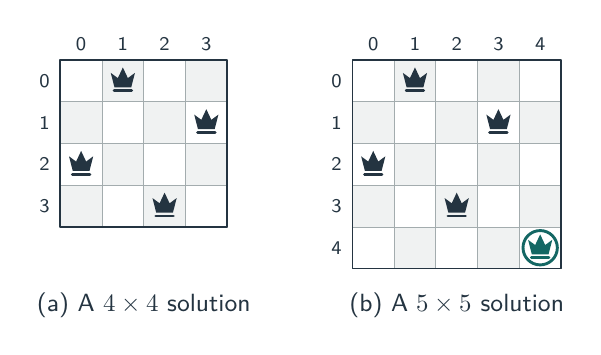
\begin{tikzpicture}[tablero A]
 \begin{scope}
  \cuadriculaA{4}\trazarRejillaA{4}
  \reinaA{0}{1}\reinaA{1}{3}\reinaA{2}{0}\reinaA{3}{2}
  \panelA{2,5.34}{(a) A $4\times4$ solution}
 \end{scope}
 \begin{scope}[shift={(7,0)}]
  \cuadriculaA{5}\trazarRejillaA{5}
  \reinaA{0}{1}\reinaA{1}{3}\reinaA{2}{0}\reinaA{3}{2}
  \aroA{4}{4}\reinaA[colorAro]{4}{4}
  \panelA{2.5,5.34}{(b) A $5\times5$ solution}
 \end{scope}
\end{tikzpicture}
\caption{Two small solutions. Each crown represents a queen. The ring marks the queen at $(4,4)$ used in the examples that follow.}
\label{fig:ejemplos}
\end{figure}


Throughout the paper we fix the board size and group placements by the number of missing queens. This
explains the word \emph{layer} in
the title. For example, removing the queen $(4,4)$ in Figure~\ref{fig:ejemplos}(b) gives a placement in
layer $h=1$ of the $5\times5$ board.
Putting it back takes us to layer $h=0$.

The same question makes sense when $h$ queens are missing. We then say that the placement has $h$
\emph{holes}. We call the set
$\Om_h(n)$ of legal placements of $n-h$ queens \emph{layer $h$}. Let $N_h(n)=|\Om_h(n)|$ and let $\mu_h$ be
the uniform law on this
layer whenever it contains at least one placement. Take a placement with law $\mu_h$. Its $h$ empty rows and
$h$ empty columns
intersect in $h^2$ \emph{empty crossings}. By the positions of the holes we shall mean the positions of
these crossings. Choose one of them
uniformly at random. We say it is \emph{available} if a queen can be added there, which is equivalent to
both of its diagonals being
free. For $h>1$, this experiment concerns the next insertion, even though some queens will still remain to
be placed.

The probability of a legal insertion can be expressed in terms of the sizes of two consecutive layers. Each
placement in layer $h-1$
has $n-h+1$ queens that we can remove individually to return to layer $h$. Conversely, each placement in
layer $h$ offers $h^2$
crossings at which to try an insertion. Counting legal insertions in both directions
(Lemma~\ref{lem:interpretacion}) shows that the
mean fraction of available crossings under $\mu_h$ is the ratio \begin{equation}\label{eq:fh}
 f_h(n)=\frac{(n-h+1)\,N_{h-1}(n)}{h^2\,N_h(n)} ,
\end{equation} which we take as the definition of $f_h(n)$ for $1\le h\le n$. Thus $f_1(n)$ answers the
question about the last queen
exactly. We prove that for each fixed $h$, $f_h(n)$ tends to the same positive constant as the board grows.

To see what is being averaged, return to Figure~\ref{fig:ejemplos}(b) and remove the queens $(1,3)$ and
$(4,4)$. With three queens left
on the $5\times5$ board, there are two holes and four crossings (Figure~\ref{fig:cruces-vacios}). The empty
rows are $1$ and $4$, and the empty
columns are $3$ and $4$. The queen at $(3,2)$ attacks $(1,4)$ along the antidiagonal with sum $5$ and
$(4,3)$ along the diagonal with
difference $1$. Each of the other two crossings can receive a queen.

\begin{figure}[htbp]
\centering
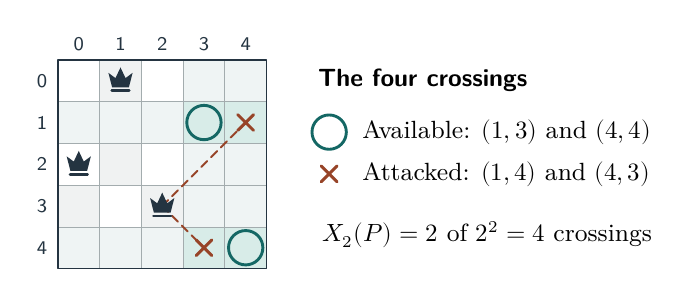
\begin{tikzpicture}[tablero A]
 \cuadriculaA{5}
 \foreach \rA in {1,4}{\fill[colorAro!7] (0,\rA) rectangle ++(5,1);}
 \foreach \cA in {3,4}{\fill[colorAro!7] (\cA,0) rectangle ++(1,5);}
 \foreach \rA in {1,4}{\foreach \cA in {3,4}{\fill[colorFondo] (\cA,\rA) rectangle ++(1,1);}}
 \trazarRejillaA{5}
 \ataqueA{3}{2}{1}{4}\ataqueA{3}{2}{4}{3}
 \reinaA{0}{1}\reinaA{2}{0}\reinaA{3}{2}
 \aroA{1}{3}\aroA{4}{4}\aspaA{1}{4}\aspaA{4}{3}
 \begin{scope}[shift={(6.0,.23)}]
  \node[anchor=west,font=\small\sffamily\bfseries] at (0,.25) {The four crossings};
  \aroA{1}{0}
  \node[anchor=west,font=\small] at (1.06,1.5) {Available: $(1,3)$ and $(4,4)$};
  \aspaA{2}{0}
  \node[anchor=west,font=\small] at (1.06,2.5) {Attacked: $(1,4)$ and $(4,3)$};
  \node[anchor=west,font=\small] at (.1,3.95) {$X_2(P)=2$ of $2^2=4$ crossings};
 \end{scope}
\end{tikzpicture}
\caption{A placement in layer $\Omega_2(5)$. The circles and crosses mark the four intersections of the
empty rows and columns. The dashed lines show why two of these squares are under attack.}
\label{fig:cruces-vacios}
\end{figure}


We write $X_h(P)$ for the number of available crossings in a placement $P$. In the example, $X_2(P)=2$, so a
uniformly chosen crossing
on this board can receive a queen with probability $2/4$. To obtain $f_2(5)$, we must average this fraction
over all legal placements
of three queens on the $5\times5$ board.

\subsection{Main results}

To identify the constant, we write $x=h/n$ for the fraction of holes. As $n$ grows with $h$ fixed, $x$ tends
to zero. This leads us to
study the full-board endpoint of the variational profile, namely the density $\nu_x$ on $[0,1]^2$ with mass
$1-x$ that maximizes the
entropy functional of Section~\ref{subsec:variacional}. For $x\in[0,1/2]$ it has the form \[
 \nu_x(r,c)=b_x\,r_{R,x}(r)\,r_{C,x}(c)\,u_{D,x}(r-c)\,u_{A,x}(r+c),
 \qquad \int_0^1 r_{R,x}=\int_0^1 r_{C,x}=1,
\] where $r_{R,x}$ and $r_{C,x}$ describe the rescaled profiles of the empty rows and columns, $u_{D,x}$ and
$u_{A,x}$ describe the
\emph{vacancies} of the diagonals and antidiagonals (the density of those that remain empty), and $b_x>0$ is
the normalization
constant. The properties of the profile are proved in~\cite{Perfil}. We define \begin{equation}\label{eq:F}
 F(x)=\frac{1-x}{b_x}=\int_{[0,1]^2}r_{R,x}(r)\,r_{C,x}(c)\,u_{D,x}(r-c)\,u_{A,x}(r+c)\,dr\,dc .
\end{equation} Heuristically, $F(x)$ is the probability that both diagonals through a typical empty crossing
are free when there are
$xn$ holes. The position of the crossing has law $r_{R,x}r_{C,x}$, and each diagonal is empty with density
$u_{D,x}$ or $u_{A,x}$
according to its direction. For the final layers the relevant constant is $F(0)=1/b_0$.

\begin{teorema}[Law of the final layers]\label{thm:limite} With the profile of Theorem~\ref{thm:perfil},
taken
from~\cite{Perfil}, for each fixed $h\ge1$, \[
 \lim_{n\to\infty}f_h(n)=F(0)=\frac1{b_0}\in(0,\infty).
\] In particular, $\max_{1\le h\le K}|f_h(n)-F(0)|\to0$ for each fixed $K$. \end{teorema}

Each factor $f_j(n)$ relates two consecutive layers. Multiplying these relations from $j=1$ to $j=h$ brings
the number of complete
solutions into the denominator.

\begin{corolario}[Ratio of layer sizes]\label{cor:cociente} For each fixed $h\ge1$, \[
 \frac{N_h(n)}{Q(n)}=\frac{(n)_h}{(h!)^2\prod_{j=1}^hf_j(n)}
 \sim\frac{n^h}{(h!)^2F(0)^h},\qquad (n)_h=n(n-1)\cdots(n-h+1).
\] \end{corolario}

Passing from layer $h$ to layer $h-1$ changes the fraction of holes from $h/n$ to $(h-1)/n$. The next
corollary uses as reference
the value of $F$ at the midpoint, $(h-\tfrac12)/n$.

\begin{corolario}[Fixed layers contribute no residual constant]\label{cor:capas} For each fixed $K$, \[
 \sum_{h=1}^K\log\frac{f_h(n)}{F\bigl((h-\tfrac12)/n\bigr)}\longrightarrow0,
\] and the same holds with $F(h/n)$ in place of $F((h-\tfrac12)/n)$. \end{corolario}

The corollary is Theorem~\ref{thm:limite} written with logarithms: each summand tends to zero because
$f_h(n)\to F(0)$ and $F$ is
continuous at $0$. Hence it does not single out the midpoint, and the conclusion holds equally with
$F(x_{n,h})$ for any
$x_{n,h}\to0$.

The number $K$ is fixed before the board size tends to infinity. Identifying the constant term of
$\log Q(n)$ would also require
control over layers whose index grows with $n$. For the final two layers we also give a direct proof of an
explicit lower bound on
$\liminf_nf_h(n)$ that does not require concentration of the reverse count (Section~\ref{sec:inversa}).

\begin{teorema}[Lower bound with an explicit constant]\label{thm:positiva} Let $\kappa\in(0,1]$ be the lower
bound on the diagonal
vacancies $u_{D,x}$ and $u_{A,x}$ of the profile of Theorem~\ref{thm:perfil}, taken from~\cite{Perfil}, and
let
$a_0=(\kappa/2)^4/16$. Then \[
 \liminf_{n\to\infty}f_h(n)\ge\frac{a_0}{2}>0,\qquad h=1,2.
\] In particular, there exist $c>0$ and $n_0$ such that $f_1(n),f_2(n)\ge c$ for all $n\ge n_0$.
\end{teorema}

Theorem~\ref{thm:limite} already implies that $\lim_nf_h(n)$ is positive for each fixed $h$. Indeed, \eqref{eq:F} and the bounds in
Theorem~\ref{thm:perfil}(a) and~(c) give $F(0)\ge\kappa^2>a_0/2$. The direct proof of Theorem~\ref{thm:positiva} is in
Section~\ref{sec:positiva}. The constant is conservative, and the proof gives only the existence of the threshold $n_0$.

To understand this proof, return to the case of the last queen. If the crossing $(r,c)$ is under attack, direct insertion there fails.
After removing a queen from $(i,j)$, we can occupy its \emph{destinations} $(r,j)$ and $(i,c)$ if the two new queens are compatible both
with the rest of the board and with each other. This fills row $r$ and column $c$ even though the crossing $(r,c)$ remains unoccupied.

For any $h\ge1$, we call this replacement of one queen by two a \emph{one-move repair} at $(r,c)$. A legal repair takes the placement
$P\in\Om_h(n)$ to layer $h-1$. Figure~\ref{fig:reparacion-tablero} shows an example on the $4\times4$ board. The queen at $(3,2)$ attacks the
empty crossing $(2,1)$. We remove the queen at $(0,0)$ and place two queens at $(2,0)$ and $(0,1)$. The original crossing remains under
attack and unoccupied. The resulting placement has four queens and is the one in Figure~\ref{fig:ejemplos}(a).

\begin{figure}[htbp]
\centering
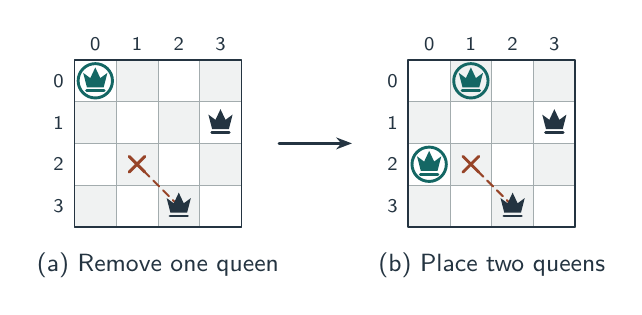
\begin{tikzpicture}[tablero A]
 \begin{scope}
  \cuadriculaA{4}\trazarRejillaA{4}
  \ataqueA{3}{2}{2}{1}\aspaA{2}{1}
  \aroA{0}{0}\reinaA[colorAro]{0}{0}\reinaA{1}{3}\reinaA{3}{2}
  \panelA{2,4.38}{(a) Remove one queen}
 \end{scope}
 \draw[-{Stealth[length=2mm]},tintaReina,line width=.9pt] (4.9,2)--(6.65,2);
 \begin{scope}[shift={(8,0)}]
  \cuadriculaA{4}\trazarRejillaA{4}
  \ataqueA{3}{2}{2}{1}\aspaA{2}{1}
  \reinaA{1}{3}\reinaA{3}{2}
  \aroA{0}{1}\reinaA[colorAro]{0}{1}
  \aroA{2}{0}\reinaA[colorAro]{2}{0}
  \panelA{2,4.38}{(b) Place two queens}
 \end{scope}
\end{tikzpicture}
\caption{A legal repair takes a placement from $\Omega_1(4)$ to $\Omega_0(4)$.
The rings mark the pieces involved. The cross marks the same square $(2,1)$ in both panels.
Reading from right to left recovers the reverse operation with the ordered pair $(2,0),(0,1)$.}
\label{fig:reparacion-tablero}
\end{figure}


We call a queen that can legally be replaced in this way an \emph{absorber} for the crossing. In
Figure~\ref{fig:reparacion-tablero}(a), only the queen at $(0,0)$ qualifies. If we remove the queen at $(1,3)$, one of its destinations is
$(1,1)$. If we remove the queen at $(3,2)$, one of its destinations is $(2,2)$. In both cases, the queen at $(0,0)$ remains in place and
attacks that destination. Thus this crossing admits no direct insertion and exactly one legal repair.

Let $A^{rc}(P)$ be the number of legal repairs at $(r,c)$ and let $d_{h,1}(P)=\sum A^{rc}(P)$, where the sum runs over the $h^2$ empty
crossings. The subscript $1$ refers to one-move repairs, in which a single queen is removed. We write $\bar r=(r+\frac12)/n$ and $\bar
c=(c+\frac12)/n$ for the coordinates of the centers of the squares. To express how the number of repairs varies with the position of the
crossing, we use the full-board profile. We denote its density by $\nu_1$, whose subscript is the mass of queens, equal to one,
corresponding to $x=0$. We drop the subscript $x$ from its factors (the constant retains its subscript, $b_0$) and set \begin{gather*}
 \nu_1=b_0\,r_R\,r_C\,u_D\,u_A,\qquad \psi(r,c)=u_D(r-c)\,u_A(r+c),\\
 a(r,c)=\int_{[0,1]^2}\nu_1(i,j)\,\psi(r,j)\,\psi(i,c)\,di\,dj .
\end{gather*} Then $\kappa^4\le a\le1$.

\begin{teorema}[Typical structure]\label{thm:estructura} Fix $h\ge1$ and let $P$ have law $\mu_h$. \begin{enumerate}[(a)] \item
\emph{One-move repairs.} In probability, \[
 \max_{(r,c)\ \text{empty crossing of }P}\ \Bigl|\frac{A^{rc}(P)}{n}-a(\bar r,\bar c)\Bigr|\longrightarrow0 .
\] \item \emph{Mean spatial distribution of the holes.} For every continuous function $t$ on $[0,1]^2$, \[
 \E_{\mu_h}\Bigl[\frac1{h^2}\sum_{(r,c)\ \text{empty crossing}}t(\bar r,\bar c)\Bigr]
 \longrightarrow\int_{[0,1]^2}t(r,c)\,r_R(r)\,r_C(c)\,dr\,dc .
\] For $h=1$ this gives weak convergence of the law of the position of the unique empty crossing. \item \emph{Unweighted counter.}
$\E_{\mu_h}[d_{h,1}]/(h^2n)\to B_1/b_0$, where $B_1=\int_{[0,1]^2}\psi$. \end{enumerate} \end{teorema}

\begin{observacion}[Scope]\label{obs:alcance} \begin{enumerate}[(i)] \item All statements hold for fixed $h$ and $K$ as $n\to\infty$.
We obtain neither convergence rates nor uniformity for $K=K(n)\to\infty$, and we do not determine the full asymptotics of $Q(n)$. \item
For $h>1$, part (b) identifies only the mean measure of the empty crossings. It makes no claim about asymptotic independence of the
empty rows and columns or concentration of the empirical measure of the empty crossings. Part (c) concerns convergence of means. By
(a), $d_{h,1}/n-\sum a(\bar r,\bar c)\to0$, and the second term may remain random, so we make no claim about concentration of
$d_{h,1}/n$. \item The value $F(0)\approx0.0809$ comes from a deterministic numerical solution of the variational
problem~\cite[Section~9]{Perfil}, with no certified error bound. At finite board sizes, the exact values from exhaustive enumeration
are far from the limit (for example $f_1(15)\approx0.114$ and $f_2(15)\approx0.153$, see Table~\ref{tab:ilustracion}). The theorem
gives no information on the rate of convergence. \end{enumerate} \end{observacion}

\subsection{Outline of the proof}\label{subsec:idea}

Figure~\ref{fig:esquema} summarizes the structure of the proof.

A placement may admit several repairs at a single crossing. We count each legal operation once from its initial placement and once from
its final placement. In the second description we start from $P'\in\Om_{h-1}$, choose the ordered pair of queens $(r,j),(i,c)$, and
replace them by $(i,j)$ to recover $P\in\Om_h$. We assign the crossing $(r,c)$ the same weight $w(r,c)$ in both descriptions. The
double count in Section~\ref{sec:doblecuenta} gives \[
 N_h\,\E_{\mu_h}D_w=N_{h-1}\,\E_{\mu_{h-1}}I_w,\qquad\text{hence}\qquad
 f_h=\frac{n-h+1}{n}\,\frac{\E_{\mu_h}[D_w/(h^2n)]}{\E_{\mu_{h-1}}[I_w/n^2]},
\] where $D_w$ and $I_w$ are the weighted forward and reverse counters. To use the ratio, we will choose a weight for which the
denominator has a positive limit.

The two means are taken under different laws, $\mu_h$ for the forward count and $\mu_{h-1}$ for the reverse count. To handle both,
Section~\ref{sec:referencia} constructs a random process for each layer $h$. It places real pieces (queens) and virtual pieces
successively until no active line remains. A virtual piece places no queen and deactivates the lines it touches. The weights come from
the variational profile. Let $\nu'_h$ denote the law of the final placement in layer $h$, conditional on the success of the process. An
entropy identity, estimates for the normalizers (the sums of weights that normalize each choice), and Simkin's first-order lower bound
give $\KL{\mu_h}{\nu'_h}=o(n)$. Consequently, an event with probability at most $e^{-cn}$ under $\nu'_h$, for fixed $c>0$, has
probability $o(1)$ under $\mu_h$.

The comparison reduces the problem to tracking repairs throughout the process. While a fixed fraction of the pieces remains, the
degrees and normalizers concentrate around their deterministic trajectories (Section~\ref{sec:regularidad}). A \emph{pattern} specifies
conditions on the squares from which queens are removed in a repair or its reverse and on the diagonals of the squares to be occupied.
Each specified square must already contain its queen or still be available, and each specified diagonal must be free of all pieces or
at least free of queens. For the forward count we track $32$ patterns for each candidate square of a crossing, and for the reverse
count we track $16$ for each pair of squares. Within each family, the expected change of a pattern can be expressed in terms of
patterns in the same family, up to an error bounded in the proof. Solving the corresponding linear system backward gives a linear
combination of patterns, the \emph{compensator}, that agrees with the counter at the chosen time and has small drift. A martingale
inequality then yields concentration up to an early cut-off, when about $\delta n$ queens remain to be placed. After the cut-off, each
queen changes the forward counter at each crossing by at most five and the reverse counter by $O(n)$. After division by $n$ and
$n^2$, respectively, the effect of the entire final stage is $O(\delta)$.

Once the loss after the cut-off has been bounded, the binary entropy inequality transfers concentration to the uniform law on each
layer. For the lower bound, the forward count suffices, since with probability tending to one every empty crossing admits at least
$a_0n/2$ repairs. To find the limit, we must take the position of the crossing into account. At $(r,c)$, the forward count concentrates
around $n\,a(\bar r,\bar c)$. Choosing the weight $w=1/a$ gives $D_{1/a}/(h^2n)\to1$. With this same weight, the mean of the reverse
counter divided by $n^2$ tends to $\int\Gamma/a$, where $\Gamma(r,c)$ is the limiting density of reverse operations that create the
crossing $(r,c)$ (Lemma~\ref{lem:nucleo}). The identity $\Gamma=b_0\,r_Rr_C\,a$, which follows from the product form of the profile,
gives $\int\Gamma/a=b_0$. Hence $f_h\to1/b_0=F(0)$. \ifverificacionLean Section~\ref{sec:verificacion} describes the Lean formalization
of the main statements and specifies what it verifies. \fi

\begin{figure}[t] \centering 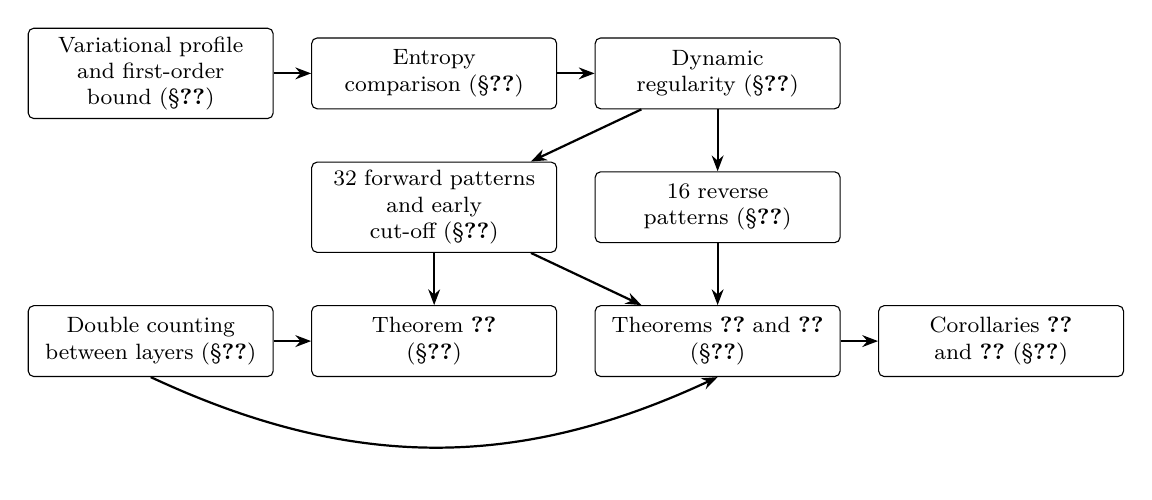
\begin{tikzpicture}[
 caja/.style={draw,rounded corners=2pt,align=center,font=\footnotesize,inner sep=3pt,
 minimum height=9mm,text width=29mm},
 flecha/.style={-{Stealth[length=2mm]},thick}]
\node[caja] (perfil) at (0,0) {Variational profile\\ and first-order bound (§\ref{sec:preliminares})};
\node[caja] (ref) at (3.6,0) {Entropy\\ comparison (§\ref{sec:referencia})};
\node[caja] (din) at (7.2,0) {Dynamic\\ regularity (§\ref{sec:regularidad})};
\node[caja] (abs) at (3.6,-1.7) {32 forward patterns\\ and early cut-off (§\ref{sec:absorbedores})};
\node[caja] (inv) at (7.2,-1.7) {16 reverse\\ patterns (§\ref{sec:inversa})};
\node[caja] (dc) at (0,-3.4) {Double counting\\ between layers (§\ref{sec:doblecuenta})};
\node[caja] (pos) at (3.6,-3.4) {Theorem~\ref{thm:positiva}\\ (§\ref{sec:positiva})};
\node[caja] (lim) at (7.2,-3.4) {Theorems~\ref{thm:limite} and~\ref{thm:estructura}\\ (§\ref{sec:limite})};
\node[caja] (cor) at (10.8,-3.4) {Corollaries~\ref{cor:cociente}\\ and~\ref{cor:capas} (§\ref{sec:corolarios})};
\draw[flecha] (perfil) -- (ref);
\draw[flecha] (ref) -- (din);
\draw[flecha] (din) -- (abs);
\draw[flecha] (din) -- (inv);
\draw[flecha] (abs) -- (pos);
\draw[flecha] (abs) -- (lim);
\draw[flecha] (inv) -- (lim);
\draw[flecha] (dc) -- (pos);
\draw[flecha] (dc.south) to[out=-25,in=-155] (lim.south);
\draw[flecha] (lim) -- (cor);
\end{tikzpicture} \caption{Logical structure of the proof. The double count is purely combinatorial. Every arrow leading to a result
under $\mu_h$ uses the entropy comparison of Section~\ref{sec:referencia}.} \label{fig:esquema} \end{figure}

\subsection{Related work}

Simkin~\cite{Simkin} characterizes the exponential term of $Q(n)$ through entropy maximization and proves a large deviation principle
for the profile of complete solutions. Earlier, Luria~\cite{Luria} obtained upper bounds using the entropy method. The first-order
lower bound we use comes from Simkin's result (Theorem~\ref{thm:simkin}). To prove it, Simkin fixes a step \emph{queenon}, that is, a
queenon (Section~\ref{sec:preliminares}) whose density is constant on each block of a grid. At each step he chooses a block with the
probability assigned to it by this measure and places a queen at random on one of its available squares. At the end he
completes the placement using absorbers~\cite[Section~5]{Simkin}. Luria and Simkin~\cite{LS} use a random greedy process to construct
near-solutions, which they complete using absorbers to obtain a counting lower bound. Bowtell and Keevash~\cite{BK} study enumeration
on the torus and its consequences for the ordinary board. The reference process and the absorbers of this paper are in the same spirit, but
success under a construction process does not by itself identify the uniform law on placements with $h$ holes; that identification
is the role of the entropy comparison. Comparing the uniform law with the output law of a random process is the main tool in Kwan's
work~\cite{Kwan} on Steiner triple systems. Double counting the repairs between consecutive layers is an instance of the method of
\emph{switchings}~\cite{McKayWormald,HMcK}.

The problem of completing a given partial placement dates back to 1850 and is NP-complete~\cite{GJN}. Glock, Munhá Correia, and
Sudakov~\cite{GMS} prove that every legal placement of at most $n/60$ queens can be completed and construct placements of size close to
$n/4$ that admit no completion. Nielsen~\cite{Nielsen} improves the upper bound on the extremal threshold to $0.216\,n$ for
sufficiently large $n$. These are worst-case results. Here we study probabilities under the uniform law on nearly complete placements.

To the best of our knowledge (our literature search was not exhaustive), Theorems~\ref{thm:limite} and~\ref{thm:estructura} and
Corollary~\ref{cor:cociente} are new. We make no claim of novelty for the general tools used here, namely the chain rule for relative
entropy, comparison with random processes~\cite{Kwan}, double counting and switchings~\cite{HMcK}, the differential equation
method~\cite{Wormald}, and concentration inequalities~\cite{AlonSpencer}.

\section{Preliminaries}\label{sec:preliminares}

\subsection{Notation}

We index the rows and columns by $\{0,\dots,n-1\}$. The square $(r,c)$ lies in row $r$, column $c$, diagonal
$r-c\in\{-(n-1),\dots,n-1\}$, and antidiagonal $r+c\in\{0,\dots,2n-2\}$. We call the rows, columns, diagonals, and antidiagonals
\emph{lines} and denote their four families by $R,C,D,A$, with $n$, $n$, $2n-1$, and $2n-1$ elements, respectively. The board is thus
a $4$-partite, $4$-uniform hypergraph whose vertices are the lines and whose edges are the squares, each consisting of its four lines.
Two distinct lines share at most one square (\emph{codegree one}). A legal placement is a matching in this hypergraph.

For $P\in\Om_h(n)$, $R_\vac(P)$ and $C_\vac(P)$ are the sets of $h$ empty rows and $h$ empty columns, respectively, and $X_h(P)$ is the
number of available empty crossings. For continuous coordinates we use the centers of the squares, $\bar r=(r+\frac12)/n$, $\bar c=(c+\frac12)/n$.
A diagonal or antidiagonal is assigned the coordinate induced by the centers of its squares, $\bar r-\bar c\in[-1,1]$ or $\bar r+\bar
c\in[0,2]$.

Unless otherwise stated, $n\to\infty$ with $h$ (or $K$) fixed. The symbols $c,C$ denote positive constants that may vary from one
occurrence to the next. Subscripts indicate dependence on fixed parameters. For laws $\mu,\nu$ on a finite set,
$\KL{\mu}{\nu}=\sum\mu\log(\mu/\nu)$ denotes relative entropy (infinite if $\mu\not\ll\nu$). We use its nonnegativity and the fact that
applying the same function to both laws cannot increase relative entropy (data processing)~\cite{CoverThomas}.

\subsection{Interpretation of \texorpdfstring{$f_h$}{fh}}

In Figure~\ref{fig:cruces-vacios} we counted the crossings in a particular placement. Summing the same counter over the entire layer
gives the following identity.

\begin{lema}\label{lem:interpretacion} For $1\le h\le n$, $\E_{\mu_h}[X_h]=h^2f_h(n)$. In particular, $f_1(n)$ is the probability that
a placement chosen uniformly from $\Om_1(n)$ can be completed to a solution. \end{lema}

\begin{proof} We count the pairs $(P,P')$ with $P\in\Om_h$, $P'\in\Om_{h-1}$, and $P\subset P'$. Each $P'$ has $n-h+1$ queens, and
removing any one of them gives a distinct $P$, yielding $(n-h+1)N_{h-1}$ pairs. Conversely, adding a queen to $P$ gives a legal
placement if and only if the queen occupies an available empty crossing, yielding $X_h(P)$ extensions. Thus
$N_h\E_{\mu_h}X_h=(n-h+1)N_{h-1}$, as claimed. If $h=1$, then $X_1\in\{0,1\}$ and $X_1(P)=1$ precisely when $P$ can be completed.
\end{proof}

\subsection{The variational problem and its profile}\label{subsec:variacional}

The preceding double count is exact at each board size. To study its limit, we need a description of the board that retains the row,
column, and diagonal constraints in continuous coordinates.

For a given mass $\rho\in(0,1]$, an \emph{admissible} density is a measurable function $\nu\ge0$ on $[0,1]^2$ with $\int\nu=\rho$ whose
projections (or marginals) onto the four families, \[
 m_R(r)=\int_0^1\nu(r,c)\,dc,\quad m_C(c)=\int_0^1\nu(r,c)\,dr,\quad
 m_D(d)=\int_{r-c=d}\nu,\quad m_A(s)=\int_{r+c=s}\nu,
\] are at most one (the last two integrate along the fiber parametrized by $r$). Its vacancies are $u_f=1-m_f$ on $I_R=I_C=[0,1]$,
$I_D=[-1,1]$, $I_A=[0,2]$. Thus $\int u_R=\int u_C=1-\rho$ and $\int u_D=\int u_A=2-\rho$. The entropy functional is \[
 s[\nu]=-3\rho-\int\nu\log\nu-\sum_{f\in\{R,C,D,A\}}\int_{I_f}u_f\log u_f ,
\] and $s^*(\rho)$ is its supremum over the admissible densities of mass $\rho$. We set $s_1=s^*(1)$. For $0<\rho<1$ the optimizer
$\nu$ is positive and satisfies the Euler equation $\nu=\lambda_\rho\,u_Ru_Cu_Du_A$ with a constant $\lambda_\rho>0$ called the
\emph{activity}~\cite[Theorem~3.1 and Lemma~3.3]{Perfil}.

With $x=1-\rho$, we rescale by setting $r_R=u_R/x$, $r_C=u_C/x$, and $b_x=\lambda_\rho x^2$, the rescaled activity. Then
\begin{equation}\label{eq:perfil}
 \nu=b_x\,r_Rr_Cu_Du_A,\qquad \int r_R=\int r_C=1,
\end{equation} and the Euler equations take the form \begin{equation}\label{eq:euler}
 r_R=\frac1{x+b_xJ_R},\quad r_C=\frac1{x+b_xJ_C},\quad
 u_D=\frac1{1+b_xJ_D},\quad u_A=\frac1{1+b_xJ_A},
\end{equation} where each $J_f$ integrates the product of the other three factors along the fiber of $f$. For example,
$J_R(r)=\int_0^1r_C(c)u_D(r-c)u_A(r+c)\,dc$. Indeed, row $r$ has mass $1-xr_R(r)=b_xr_R(r)J_R(r)$. Integrating~\eqref{eq:perfil} gives
expression~\eqref{eq:F} for $F(x)=(1-x)/b_x$. We write $\nu_x$ and $(b_x,r_{R,x},r_{C,x},u_{D,x},u_{A,x})$ when we need to specify $x$.
The subscript then denotes the fraction of holes, not the mass (in~\cite{Perfil} the densities are indexed by mass, so our $\nu_x$ is denoted there
by $\nu_{1-x}$). The sole exception is the density of mass one, corresponding to $x=0$, which we denote by $\nu_1$ as in~\cite{Perfil}.

\begin{teorema}[The profile near the full board~\cite{Perfil}]\label{thm:perfil} There exist constants $0<\kappa\le1$, $0<\underline
r\le M<\infty$, $0<b_-\le b_+<\infty$, and $L_*<\infty$ such that for all $x\in(0,1/2]$ the optimal profile of mass
$1-x$~\cite[Theorem~3.1]{Perfil}, rescaled as in~\eqref{eq:perfil}, satisfies~\eqref{eq:euler} and the following properties.
\begin{enumerate}[(a)] \item $b_-\le b_x\le b_+$, $\ \underline r\le r_{R,x},r_{C,x}\le M$, and $\kappa\le u_{D,x},u_{A,x}\le1$. \item
$r_{R,x},r_{C,x},u_{D,x},u_{A,x}$ are Lipschitz on their respective intervals with Lipschitz constant at most $L_*$, and $\nu_x$ is
bounded and Lipschitz, uniformly in $x$. \item As $x\downarrow0$ they converge uniformly to limits $(b_0,r_R,r_C,u_D,u_A)$
satisfying~\eqref{eq:euler} with $x=0$ and the same bounds. \end{enumerate} In particular, $\nu_1=b_0r_Rr_Cu_Du_A$ is a continuous
density on $[0,1]^2$ of mass one, with row and column marginals equal to one and diagonal vacancies $u_D=1-m_D$ and $u_A=1-m_A$, so
$\int u_D=\int u_A=1$; $\nu_1$ is the unique maximizer of $s$ among admissible densities of mass one, so that
$s[\nu_1]=s^*(1)=s_1$; and $F$ is continuous at $0$ with $F(0)=1/b_0>0$. \end{teorema}

Parts (a) and (c) are Propositions~4.2, 5.2, and~5.3 of~\cite{Perfil}. The assertion that the limit $\nu_1$ is the unique maximizer of
mass one follows from Propositions~5.1 and~5.2 of that work. Uniform Lipschitz regularity (b) is its Theorem~7.7, and continuity of $F$
at $0$, with $F(0)=1/b_0$, is its Theorem~8.1. Appendix~\ref{app:perfil} summarizes those proofs and gives explicit values for the
constants. No identification of the profile with discrete laws on placements is used:
Theorem~\ref{thm:perfil} is a statement about the continuous problem.

\subsection{Simkin's first-order estimate}

\begin{teorema}[{Consequence of~\cite[Theorem~2.11]{Simkin}}]\label{thm:simkin}
$\log Q(n)\ge n\log n+ns_1-o(n)$, with $s_1=s^*(1)=s[\nu_1]$. \end{teorema}

Theorem~2.11 of~\cite{Simkin} is stated for \emph{queenons}~\cite[Definitions~2.1, 2.3 and~2.4]{Simkin},
which form the weak closure of
the step permutons with subuniform diagonal marginals. After translating the square to
$[-\frac12,\frac12]^2$, a density whose row and
column marginals equal one defines a permuton, and the diagonal marginals are subuniform precisely when
$m_D,m_A\le1$.

\begin{lema}\label{lem:queenon} The measure with density $\nu_1$, translated to $[-\frac12,\frac12]^2$, is a
queenon. \end{lema}

\begin{proof} By Theorem~\ref{thm:perfil}, $\nu_1$ is continuous on the closed square, has row and column
marginals equal to one, and
has diagonal projections satisfying $m_D=1-u_D\le1-\kappa$ and $m_A=1-u_A\le1-\kappa$. For $N\ge1$, let
$\nu^{(N)}$ be the density
whose value on each cell of the $N\times N$ grid is the average of $\nu_1$ over that cell. On a horizontal
strip of width $1/N$, the
row marginal of $\nu^{(N)}$ is the average of the row marginal of $\nu_1$, which equals one. The same holds
for the columns, so
$\nu^{(N)}$ is a step permuton. If $\omega$ is the modulus of uniform continuity of $\nu_1$, then
$|\nu^{(N)}-\nu_1|\le\omega(\sqrt2/N)$ and, since the diagonal fibers have parametric length (in $r$) at
most one,
$m_D[\nu^{(N)}],m_A[\nu^{(N)}]\le1-\kappa+\omega(\sqrt2/N)\le1$ for sufficiently large $N$. This is the
normalization used
in~\cite{Simkin}. The pushforward of the measure under $(r,c)\mapsto r\mp c$ has density given by the fiber
integral in $r$ because the
Jacobian is one. Thus $\nu^{(N)}$ has subuniform diagonal marginals and converges uniformly to $\nu_1$,
hence in total variation and in
particular weakly. \end{proof}

\begin{proof}[Proof of Theorem~\ref{thm:simkin}] By Lemma~\ref{lem:queenon}, Theorem~2.11 of~\cite{Simkin}
applies to $\nu_1$
as stated. There is no need to invoke Remark~2.7 there,
which extends the theorem to all permutons with subuniform diagonal marginals. After translation, the
diagonal vacancy densities are
$u_D,u_A$, each with integral one. In Definition~2.9 of~\cite{Simkin}, each divergence from the uniform law
on $[-1,1]$ equals $\int
u\log
u+\log2$, and the two constants cancel with $2\log2$. Simkin's functional at $\nu_1$ is therefore
$-3-\int\nu_1\log\nu_1-\int
u_D\log u_D-\int u_A\log
u_A=s[\nu_1]=s_1$. The lower bound in his Theorem~2.11 for this profile yields the claim. First fix the
tolerance, then take the limit inferior in $n$, and finally let the tolerance tend to zero. \end{proof}

This argument gives no rate for the remainder, and we write \begin{equation}\label{eq:Delta}
 \Delta_n=\bigl[n\log n+ns_1-\log Q(n)\bigr]_+=o(n).
\end{equation}

Simkin also proves the matching upper bound~\cite[Theorem~1.1]{Simkin}, and the maximum of his functional
over queenons is the
negative of his constant $\alpha\in(1.94,\,1.9449)$~\cite[Section~2]{Simkin}. By the same computation, this
functional equals $s[\nu]$
at a queenon with density $\nu$, which is admissible of mass one, and equals $-\infty$ at all other
queenons. Since $\nu_1$ maximizes
$s$ at mass one, $s_1$ is this maximum; that is, $-s_1$ is the constant $\alpha$ of~\cite{Simkin} and
$\log Q(n)=n\log n+ns_1+o(n)$. Nobel, Agrawal and Boyd~\cite{NAB} obtain, with floating-point computations
and without
certification, $1.944000752\le-s_1\le1.944001082$.

\subsection{The variational value near the full board}

\begin{lema}\label{lem:borde} As $x\downarrow0$, $s^*(1-x)-s^*(1)=2x\log(1/x)+O(x)$. Consequently, for fixed
$K$ and $0\le h\le K$, \[
 n\bigl[s^*(1-h/n)-s_1\bigr]=2h\log n+O_K(1).
\] \end{lema}

This is Proposition~8.3 of~\cite{Perfil}, where the supporting-line inequality (Theorem~3.1(d), with
$\theta=-\log\lambda_\rho$) and the continuity of $s^*$ at $\rho=1$ (Proposition~5.1) are also proved. We
include the proof for completeness.

\begin{proof} The functional $s$ is concave on the admissible domain. At a positive profile
$\nu=\lambda_\rho\prod_fu_f$, its
derivative in the direction of an admissible variation $\dot\nu$ with $\int\dot\nu=\dot\rho$ is \[
 \dot s=\int\Bigl[-3-1-\log\nu+\sum_f(1+\log u_f)\Bigr]\dot\nu=-\log\lambda_\rho\;\dot\rho ,
\] since $-\log\nu+\sum_f\log u_f=-\log\lambda_\rho$ and $-3-1+4=0$. Concavity and stationarity at fixed
mass identify the value
$s^*(\rho)$ and give the supporting-line inequality \[
 s^*(\rho')\le s^*(\rho)-\log\lambda_\rho\,(\rho'-\rho).
\] On compact subintervals of $(0,1)$, $s^*$ is concave and hence absolutely continuous. At its points of
differentiability, the
supergradient $-\log\lambda_\rho$ equals its derivative. The two-sided bounds on
$b_x=\lambda_\rho(1-\rho)^2$ give
$-\log\lambda_\rho=2\log(1-\rho)+O(1)$. By Theorem~\ref{thm:perfil}(c) and continuity of $u\log u$, the
optimal value at mass $1-x$
tends to $s[\nu_1]$, which equals $s^*(1)$ because $\nu_1$ is the maximizer of mass one
(Theorem~\ref{thm:perfil}). This proves
continuity of $s^*$ at $\rho=1$. Together with the integrability of $\log(1-\rho)$, this allows us to
integrate, giving \[
 s^*(1)-s^*(1-x)=\int_{1-x}^1\bigl[2\log(1-\rho)+O(1)\bigr]d\rho=2x\log x-2x+O(x).
\] This proves the first assertion. The second follows on setting $x=h/n$, which gives
$n[2(h/n)\log(n/h)+O(h/n)]=2h\log n+O_K(1)$. \end{proof}

The argument uses only concavity and does not differentiate the profile with respect to its parameter.

\subsection{Two relative entropy lemmas}

\begin{lema}[Conditioning on success]\label{lem:exito} Let $\PP,\QQ$ be laws on a finite set and let $S$ be
an event with $\PP(S)=1$
and $\QQ(S)>0$. Then $\KL{\PP}{\QQ(\cdot\mid S)}=\KL{\PP}{\QQ}+\log\QQ(S)$. In particular,
$\QQ(S)\ge e^{-\KL{\PP}{\QQ}}$ and
$\KL{\PP}{\QQ(\cdot\mid S)}\le\KL{\PP}{\QQ}$. \end{lema}

\begin{proof} On $S$, $\QQ(\omega\mid S)=\QQ(\omega)/\QQ(S)$. Take the expectation of
$\log(\PP/\QQ(\cdot\mid
S))=\log(\PP/\QQ)+\log\QQ(S)$ under $\PP$. Nonnegativity of the left-hand side gives both consequences.
\end{proof}

\begin{lema}[Binary transfer]\label{lem:binaria} Let $\mu,\nu$ be laws on a finite set and let $B$ be an
event with $\nu(B)<1$. Then \[
 \mu(B)\log\frac1{\nu(B)}\le\KL{\mu}{\nu}+\log2 .
\] If $\nu(B)=0$ and $\KL{\mu}{\nu}<\infty$, then $\mu(B)=0$. \end{lema}

\begin{proof} Let $p=\mu(B)$ and $p'=\nu(B)$. Applying data processing to the indicator of $B$ gives \[
\begin{aligned}
 \KL{\mu}{\nu}&\ge p\log\frac p{p'}+(1-p)\log\frac{1-p}{1-p'}\\
 &\ge p\log\frac1{p'}+p\log p+(1-p)\log(1-p)\ge p\log\frac1{p'}-\log2 .
\end{aligned}
\] The case $p'=0$ follows from absolute continuity. \end{proof}

In Sections~\ref{sec:regularidad}--\ref{sec:inversa} we also use the Azuma--Hoeffding inequality for
martingales with bounded
increments~\cite{AlonSpencer} and the discrete Gronwall inequality in the usual form used in the
differential equation
method~\cite{Wormald,Warnke,BennettDudek}.

\section{Reference process and entropy comparison}\label{sec:referencia}

The continuous profile supplies the weights for constructing placements one step at a time. This section
compares the law of the
resulting placements, conditional on success, with the uniform law on the layer. The relative entropy bound
will allow us to transfer
estimates obtained during the construction to the uniform law.

Fix $K$ and $0\le h\le K$, and set \[
 q=n-h,\qquad N=2n-1,\qquad H=N-q=n+h-1 .
\] In this section and the next two, for $h\ge1$ we evaluate the profile at the target parameter $x_*=h/n$,
which is held fixed
throughout the process, and omit the subscript $x_*$. Where this target profile and the full-board profile
appear together, as in
Section~\ref{subsec:trayectoria}, we write the subscript $x_*$ again on the former. We treat layer $h=0$
separately in
Section~\ref{subsec:h0}.

\subsection{Augmented hypergraph and weights}

We add $n-1$ \emph{dummy} vertices to the rows and as many to the columns, so that each of the four families
contains $N$ vertices. The
\emph{real edges} are the $n^2$ squares, each with its four physical lines. The \emph{virtual edges} are all
quadruples containing one
vertex from each family, whether physical or dummy. The color (real or virtual) is part of the edge. A
virtual edge is distinct from a
real edge even if they have the same vertices.

In Figure~\ref{fig:cruces-vacios}, the lines through $(3,2)$ are $R_3$, $C_2$, $D_1$, and $A_5$ because
$3-2=1$ and $3+2=5$. Choosing
the real edge on that square places a queen there. Choosing the virtual edge with the same four lines
deactivates those lines in the
process without placing a queen on the board. We will use this distinction when counting repairs. We call
the edges in a trajectory
\emph{pieces}. These are the edges chosen by the process, real or virtual according to their color.

For $h\ge1$, the vertex weights are $u_R(\bar r)=x_*r_R(\bar r)$ on the physical rows,
$u_C(\bar c)=x_*r_C(\bar c)$ on the physical
columns, $u_D$ and $u_A$ at the induced coordinates of the diagonals and antidiagonals, respectively, and
$1$ on the dummy vertices.
All weights are positive. The weight of an edge, real or virtual, is the product
$\varpi(e)=\prod_{v\in e}u_v$. By
Theorem~\ref{thm:perfil}(a), every real edge has weight between $cx_*^2$ and $Cx_*^2$.

\subsection{The process}

\begin{definicion}[Reference process]\label{def:referencia} Choose in advance, without revealing it, a
uniformly random word with $q$
occurrences of the real color and $H$ of the virtual color. At each step $t=1,\dots,N$, reveal only the next
color, choose an available
edge of that color (one whose four vertices are still active) with probability proportional to its weight,
and deactivate its four
vertices. A virtual piece places no queen. If the normalizer for the requested color, namely the sum of the
weights of its available
edges, is zero, the process enters a failure state. Let $\QQ_h$ be the law of the trajectories and $S$ the
success event (all $N$ steps
are completed). \end{definicion}

On $S$, the $q$ selected real edges are squares with no lines in common. They form a placement in
$\Om_h(n)$, called the \emph{final
placement}. Let $\nu'_h$ be its law under $\QQ_h(\cdot\mid S)$. For real choices the common factor $x_*^2$
can be cancelled without
changing the law; it does not cancel for virtual choices. The reference process need not succeed with
probability close to one.

\subsection{The comparison law}

\begin{definicion}[Comparison law]\label{def:comparacion} Choose $P\in\Om_h(n)$ uniformly at random, then
choose a uniform virtual
completion, that is, a perfect matching by virtual edges of the $H$ free vertices in each family (there are
$(H!)^3$ such matchings).
Finally, choose a uniform ordering of the $N$ pieces. Let $\PP_h$ be the law of the resulting sequence of
edges. \end{definicion}

We represent the uniform order by assigning the pieces independent uniform times in $[0,1]$ and revealing
them in increasing order of
time. (This uses independence. Uniformity of each individual time would not suffice.) These independent
times, together with
Jensen's inequality in Lemma~\ref{lem:normalizadores}(iii), are the device of the entropy bounds of
Radhakrishnan~\cite{Radhakrishnan} and of Linial and Luria~\cite{LinialLuria}. The law $\PP_h$ projects
exactly onto $\mu_h$, and
each trajectory in its support has positive probability under $\QQ_h$ because the next piece of the complete
matching remains available
and has positive weight. In particular, $\PP_h(S)=1$.

\subsection{The entropy identity}

Let $W_R(t)$ and $W_V(t)$ be the total weights of the available edges of the two colors before step $t$, and
let $\col(t)$ denote the
color revealed at that step.

\begin{lema}\label{lem:identidad} For $1\le h\le K$, \[
 \KL{\PP_h}{\QQ_h}=\E_{\PP_h}\sum_{t=1}^N\log W_{\col(t)}(t)-\sum_v\log u_v-\log N_h-\log q!
 -4\log H!,
\] where $\sum_v$ ranges over the $4N$ vertices. \end{lema}

\begin{proof} Let $\omega$ be a trajectory in the support of $\PP_h$. Then
$\PP_h(\omega)=[N_h(H!)^3N!]^{-1}$. Under $\QQ_h$, the color
word has probability $\binom Nq^{-1}$ and each choice has probability $\varpi(e_t)/W_{\col(t)}(t)$. Since
the complete matching covers
every vertex exactly once, the product of the chosen weights is $\prod_vu_v$, independent of the matching
and its order. Hence \[
 \log\frac{\PP_h(\omega)}{\QQ_h(\omega)}=\sum_t\log W_{\col(t)}(t)-\sum_v\log u_v
 -\log\bigl[N_h(H!)^3N!\bigr]+\log\binom Nq ,
\] and $-\log[(H!)^3N!]+\log\binom Nq=-\log q!-4\log H!$. Taking the expectation under $\PP_h$ gives the
result. \end{proof}

\subsection{Normalizers}

\begin{lema}\label{lem:normalizadores} Let $\rho=1-x_*=q/n$. The following hold uniformly in $1\le h\le K$. \begin{enumerate}[(i)]
\item $W_R(0)=n^2\rho/\lambda_\rho\,(1+O(n^{-1}))\asymp x_*^2n^2$ and $W_V(0)=H^4(1+O(n^{-1}))$. \item $\sum_v\log
u_v=n\sum_f\int_{I_f}\log u_f+O(1)$. \item $\E_{\PP_h}\sum_t\log W_{\col(t)}(t)\le q\log W_R(0)+H\log W_V(0)-4N+O(n^{2/3})$.
\end{enumerate} \end{lema}

\begin{proof} (i) By quadrature for the rescaled factors, which are positive and Lipschitz, $W_R(0)=x_*^2n^2\int
r_Rr_Cu_Du_A\,(1+O(n^{-1}))=x_*^2n^2\rho/b\,(1+O(n^{-1}))$; moreover $x_*^2/b=1/\lambda_\rho$. In each family the sum of the weights is
$H+O(1)$. For the rows we sum $n-1$ dummy contributions and $\sum u_R=nx_*+O(x_*)$. For the diagonals the sum is $\sum u_D=n\int
u_D+O(1)=n(2-\rho)+O(1)$. Since $W_V(0)$ is the product of the four sums, $W_V(0)=H^4(1+O(n^{-1}))$.

(ii) For the rows, $\sum\log u_R=n\log x_*+\sum\log r_R(\bar r)$. The constant $\log x_*$ is summed exactly $n$ times, and $\log r_R$
is uniformly Lipschitz, so the quadrature error is $O(1)$ independently of $1/x_*$. The same holds for the columns, diagonals, and
antidiagonals. The dummy vertices contribute zero.

(iii) Fix a completed matching and a piece $p$ revealed at time $\mathsf t_p\in[0,1]$. Let $z=1-\mathsf t_p$, and let $W^{(p)}$ denote
the normalizer for the color of $p$ at the time it is revealed. Conditional on the matching and on $\mathsf t_p$, each of the other
pieces independently remains unrevealed with probability $z$. An \emph{ordinary} edge of the color of $p$ has its four vertices covered
by four distinct pieces other than $p$ and is available with probability $z^4$. By the codegree-one property there are $O(n)$
exceptional real edges of weight $O(x_*^2)$. Except for the one contained in $p$, each requires at least one other piece to remain
unrevealed and is available with probability at most $z$. There are $O(n^3)$ exceptional virtual edges, each of weight at most one.
Thus, uniformly in the matching, \[
 \E W^{(p)}\le W_R(0)z^4+Cx_*^2nz+Cx_*^2\ \ (p\text{ real}),\qquad
 \E W^{(p)}\le W_V(0)z^4+Cn^3z+C\ \ (p\text{ virtual}).
\] By Jensen's inequality, (i), and $\log(1+u+v)\le\log(1+u)+\log(1+v)$, the error terms are of orders $1/(nz^3)$ and $1/(n^2z^4)$ for
real $p$ and $1/(nz^3)$ and $1/(n^4z^4)$ for virtual $p$. Since $\int_0^1\log z^4\,dz=-4$ and, for fixed $c>0$,
$\int_0^1\log(1+cn^{-1}z^{-3})\,dz=O(n^{-1/3})$, $\int_0^1\log(1+cn^{-2}z^{-4})\,dz=O(n^{-1/2})$, and
$\int_0^1\log(1+cn^{-4}z^{-4})\,dz=O(n^{-1})$, we obtain \[
 \E\log W^{(p)}\le\log W_{\col(p)}(0)-4+O(n^{-1/3}).
\] Since $\sum_t\log W_{\col(t)}(t)=\sum_p\log W^{(p)}$, summing over the $N$ pieces gives (iii). \end{proof}

\begin{lema}\label{lem:retirada}
$N_h(n)\ge\binom nh Q(n)/h!$.
\end{lema}

\begin{proof} Removing $h$ queens from a solution gives a placement in $\Om_h$, and each placement in $\Om_h$ has at most $h!$
completions, because the $h$ missing queens occupy a permutation of the $h$ empty crossings. Hence $\binom nhQ\le h!N_h$. \end{proof}

\begin{teorema}[Entropy comparison]\label{thm:comparacion} Fix $K$. There exists $d_n=\Delta_n+C_Kn^{2/3}+O_K(\log n)=o(n)$ such that
for all $0\le h\le K$, \[
 \KL{\PP_h}{\QQ_h}\le d_n,\qquad \QQ_h(S)\ge e^{-d_n},\qquad \KL{\mu_h}{\nu'_h}\le d_n .
\] \end{teorema}

\begin{proof}[Proof for $1\le h\le K$] By Lemmas~\ref{lem:identidad} and~\ref{lem:normalizadores} and Stirling's formula ($\log
H!=H\log H-H+O(\log n)$, and likewise for $q!$), \[
 \KL{\PP_h}{\QQ_h}\le q\log\frac{n^2\rho}{\lambda_\rho}-4q-n\sum_f\int\log u_f-(q\log q-q)
 -\log N_h+Cn^{2/3}+O(\log n),
\] where we have used $4H\log H-4\log H!=4H+O(\log n)$ and $N-H=q$. With $q=n\rho$, we have $q\log(n^2\rho)-q\log q=q\log n$, so the
right-hand side is $q\log n+n[-3\rho-\rho\log\lambda_\rho-\sum_f\int\log u_f]-\log N_h+Cn^{2/3}+O(\log n)$. The expression in brackets
is $s^*(\rho)$, since the Euler equation gives $\int\nu\log\nu=\rho\log\lambda_\rho+\sum_f\int m_f\log u_f$ and $\int m_f\log
u_f=\int\log u_f-\int u_f\log u_f$. Thus \[
 \KL{\PP_h}{\QQ_h}\le q\log n+ns^*(q/n)-\log N_h+Cn^{2/3}+O(\log n).
\] By Lemma~\ref{lem:borde}, $ns^*(q/n)=ns_1+2h\log n+O_K(1)$. By Lemma~\ref{lem:retirada}, $-\log N_h\le-\log Q-\log\binom nh+\log
h!=-\log Q-h\log n+O_K(1)$. The terms in $\log n$ cancel exactly ($-h+2h-h=0$), and by~\eqref{eq:Delta},
$\KL{\PP_h}{\QQ_h}\le\Delta_n+C_Kn^{2/3}+O_K(\log n)=d_n$. No rate is needed for $\Delta_n$. Since $\PP_h(S)=1$, Lemma~\ref{lem:exito}
gives $\QQ_h(S)\ge e^{-d_n}$ and $\KL{\PP_h}{\QQ_h(\cdot\mid S)}\le d_n$. Projecting onto the final placement and applying data
processing gives $\KL{\mu_h}{\nu'_h}\le d_n$. \end{proof}

\subsection{Layer zero}\label{subsec:h0}

At $h=0$ the weights $x_*r_R$ of the physical rows and columns vanish, so direct substitution of $x_*=0$ in
the preceding construction
is impossible. We use an explicit limiting extension.

\begin{definicion}[Reference process in layer zero]\label{def:referencia_cero} Let $q=n$, $H=n-1$, $N=2n-1$.
The real edges have weight
$v_e=r_Rr_Cu_Du_A$, evaluated at the full-board profile. The vertex weights for virtual edges are zero on
physical rows and columns,
one on their dummy vertices, and $u_D,u_A$ on diagonals and antidiagonals. The color word is still uniform,
and the process enters the
failure state if there is no edge of the requested color. The laws $\QQ_0$, $\PP_0$, and $\nu'_0$ are
defined as before.
\end{definicion}

\begin{proof}[Proof of Theorem~\ref{thm:comparacion} for $h=0$] \emph{Support.} Every solution uses all
physical rows and columns, so
its virtual completions use only dummy row and column vertices. Thus every trajectory in the support of
$\PP_0$, the uniform law on
solutions, completions, and orders, has positive probability under $\QQ_0$ despite the zero weights outside
this support.

\emph{Identity.} The product of the weights along any trajectory in this support is \[
 \mathcal K=\prod_{R}r_R\prod_{C}r_C\prod_{D}u_D\prod_{A}u_A>0
\] (products over the physical vertices). There are $Q(H!)^3N!$ comparison trajectories, and the color word
has probability exactly
$n!H!/N!$. Hence \[
 \KL{\PP_0}{\QQ_0}=\E\sum_t\log W_{\col(t)}(t)-\log\mathcal K-\log Q-\log n!-4\log H! .
\] The term $\log0$ does not appear.

\emph{Normalizers.} For the Lipschitz full-board profile, the masses give \[
 W_R(0)=\frac{n^2}{b_0}\bigl(1+O(n^{-1})\bigr),\qquad
 W_V(0)=H^2\Bigl(\sum_Du_D\Bigr)\Bigl(\sum_Au_A\Bigr)=H^4\bigl(1+O(n^{-1})\bigr),
\] since $\int u_D=\int u_A=1$ on domains of length two and each discrete sum is $n\int+O(1)$. Likewise,
$\log\mathcal K=n\mathcal
J+O(1)$ with $\mathcal J=\int\log r_R+\int\log r_C+\int\log u_D+\int\log
u_A$. As a completed matching is revealed, ordinary edges
survive with probability $z^4$. There are $O(n)$ exceptional real edges of weight $O(1)$ and $O(n^3)$
exceptional virtual edges of
weight at most one (by the count in the proof of Lemma~\ref{lem:normalizadores}(iii)). Except for the piece
itself, each requires another piece to remain unrevealed. The zero virtual weights merely set
some terms of the virtual normalizer to zero. As in Lemma~\ref{lem:normalizadores}, Jensen's inequality
gives an integrated error of
$O(n^{-1/3})$ per piece. By Stirling's formula and $s_1=-3-\log b_0-\mathcal J$ (which is $s[\nu_1]$
evaluated with
$\nu_1=b_0r_Rr_Cu_Du_A$ and with row and column marginals equal to one), we obtain \[
 \KL{\PP_0}{\QQ_0}\le n\log n+ns_1-\log Q+Cn^{2/3}+O(\log n)\le d_n .
\] The other two inequalities follow as for $h\ge1$. \end{proof}

\begin{observacion} The proof for $1\le h\le K$ is uniform in $h$. It uses only $x_*=h/n$, cancellation of
the factor $x_*^2$,
Lemma~\ref{lem:retirada}, and Lemma~\ref{lem:borde}. The same $d_n$ works simultaneously for $h=0,\dots,K$.
This gives no uniformity
when $K=K(n)\to\infty$. \end{observacion}

\section{Dynamic regularity of the process}\label{sec:regularidad}

The entropy comparison already allows us to transfer sufficiently rare events. To apply it to repairs, we
first need to know how often
the process selects the lines that the two queens in a repair would occupy. These probabilities depend on
the weights and the available
degrees at each step.

\subsection{Rescaled weights and initial balance}

For $1\le h\le K$ we rescale only the real weights by the common factor $x_*^{-2}$, which leaves the law
unchanged, giving
$v_e=\varpi(e)/x_*^2=r_Rr_Cu_Du_A$. For $h=0$, $v_e$ is the real weight from
Definition~\ref{def:referencia_cero} itself. By
Theorem~\ref{thm:perfil}(a), $c\le v_e\le C$ with $c=\underline r^2\kappa^2$ and $C=M^2$. Set \[
 W_0=\sum_ev_e\asymp n^2,\quad \deg_v^0=\sum_{e\ni v}v_e,\quad \pi_e=\frac{qv_e}{W_0},\quad
 p_v=\sum_{e\ni v}\pi_e,\quad U_f^0=\sum_{v\in f}u_v .
\] We retain the virtual weights $u_v$. The dummy vertices have $u_v=1$ and $p_v=0$.

\begin{lema}[Initial balance]\label{lem:balance} Uniformly in $0\le h\le K$, for every physical vertex $v$
and every real edge $e$,
\begin{equation}\label{eq:balance}
 p_v+u_v=1+O(n^{-1}),\qquad U_f^0=H+O(1),\qquad p_v\le C,\qquad \pi_e\le C/n .
\end{equation} Moreover, $\sum_{v\in f}p_v=q$ in each family, and for diagonals and antidiagonals,
$p_v\le1-\eta$ with $\eta=\kappa/2$,
for $n$ large. \end{lema}

\begin{proof} Let $\rho_n=q/n$. By quadrature, $W_0=n^2\rho_n/b\,(1+O(n^{-1}))$. On a row $r$, the Euler
equation~\eqref{eq:euler} gives
$q\deg_v^0/W_0=b\,r_R(\bar r)J_R(\bar r)+O(n^{-1})=1-u_R+O(n^{-1})$. On a diagonal,
$q\deg_v^0/W_0=b\,u_DJ_D+O(n^{-1})=1-u_D+O(n^{-1})$. The arguments for columns and antidiagonals are
analogous. The bounds and
quadrature estimates are uniform up to the boundary of the target profile. Each real edge appears exactly
once in each family, so
$\sum_{v\in f}\deg_v^0=W_0$ and $\sum_{v\in f}p_v=q$. Summing the pointwise balance gives
$U_f^0=N-q+O(N/n)=H+O(1)$, including the
dummy vertices. On diagonals, $u_v\ge\kappa$, whence $p_v\le1-\kappa+O(n^{-1})\le1-\eta$. At $h=0$ the
balance is $p_v=1+O(n^{-1})$,
with $u_v=0$ on physical rows and columns. The sum of the virtual weights in each of these families is $H$
(from dummy vertices alone),
and the diagonals are unchanged. \end{proof}

\emph{Clocks.} The index $t$ counts all pieces placed, $z_t=(N-t)/N$ is the active fraction, and $q_t$ is
the number of real pieces still to be
placed. Neither $z_t$ nor $q_t/n$ replaces the fixed parameter $x_*$ in the weights.

\section{Absorbers: forward patterns and early cut-off}\label{sec:absorbedores}

Fix $1\le h\le K$ and work under $\QQ_h$. We track the queens that could be removed to make a repair at a given crossing. The degree
estimates from the preceding section allow us to estimate how their number changes when the next piece is placed.

\subsection{Repairs at a crossing and line marks}

The \emph{root} is the square $(r,c)$ that we track as a possible empty crossing. In Figure~\ref{fig:reparacion-tablero} it would be
$(2,1)$. The candidate queen occupies $(0,0)$ and its two \emph{destinations} are $(2,0)$ and $(0,1)$. We first check that the destinations are
compatible with each other. We call this condition the $G$ filter. We then check that the diagonals of both destinations are free of other
queens.

Fix a root $(r,c)$. Let $\mathcal I_{rc}$ be the set of squares $e=(i,j)$ with $i\ne r$ and $j\ne c$ whose \emph{destinations} $(r,j)$ and
$(i,c)$ do not attack each other (filter $G=1$). This excludes at most $Cn$ squares. The \emph{candidates} for the root are the
squares in $\mathcal I_{rc}$. Candidates that contain a queen are called \emph{occupied}. The four lines of $e$ and the four diagonals
and antidiagonals of its destinations are eight distinct vertices. This is where we use the $G$ filter. We denote the latter four lines by
$d_1,\dots,d_4$ and their list by $\mathcal D(r,c;i,j)$.

For a vertex $v$, let $\chi_v$ indicate that $v$ is active and let $V_v$ indicate that line $v$ is physically free of queens. We always
have $\chi_v\le V_v$. The \emph{mark} of a line $v$ is its state: the line carries the active mark if $\chi_v=1$ and the mark $V$ if $V_v=1$. Let
$O_e$ indicate that a real queen has been placed at $e$, and let $\chi_e=\prod_{v\in e}\chi_v$. For $J\subseteq\{1,2,3,4\}$ set
\begin{equation}\label{eq:patrones}
 M_J=\prod_{i\in J}\chi_{d_i}\prod_{i\notin J}V_{d_i},\qquad
 Z^\oc_{e,J}=O_e\,M_J,\qquad Z^\di_{e,J}=\chi_e\,M_J .
\end{equation} There are $32$ patterns per square, and apart from the remainder terms in Lemma~\ref{lem:generador}, the process
generates no others. The extended physical counter is \[
 A^{rc}=\sum_{e\in\mathcal I_{rc}}Z^\oc_{e,\varnothing}=\sum_{e\in\mathcal I_{rc}}O_e\prod_{i=1}^4V_{d_i}.
\] If row $r$ and column $c$ are physically empty, $A^{rc}$ equals the number of legal one-move repairs at crossing $(r,c)$. Indeed,
removing the queen at $e$ and placing queens at its two destinations is legal exactly when the four destination diagonals are empty. The rescaled
weighted availability is $\overline Y^{rc}=\sum_{e\in\mathcal I_{rc}}v_eZ^\di_{e,\varnothing}$. With the original weights it is
$x_*^2\overline Y^{rc}$.

\subsection{Reference generator}

In discrete time, with $z=(N-t)/N$, define \[
 \alpha=\frac1{Nz},\qquad \beta_i=\frac{p_{d_i}}{Nz},\qquad k_e=\frac{\pi_e}{Nz^4},
\] and the linear operator \begin{equation}\label{eq:generador}
\begin{aligned}
 \cL Z^\oc_{e,J}&=-|J|\,\alpha\,Z^\oc_{e,J}-\sum_{i\notin J}\beta_i\,Z^\oc_{e,J\cup\{i\}}+k_e\,Z^\di_{e,J},\\
 \cL Z^\di_{e,J}&=-(4+|J|)\,\alpha\,Z^\di_{e,J}-\sum_{i\notin J}\beta_i\,Z^\di_{e,J\cup\{i\}} .
\end{aligned}
\end{equation} An active mark dies at rate $\alpha$ when hit by a real or virtual piece. A mark $V$ dies only when hit by a real piece,
which requires the corresponding active mark. This turns $V_{d_i}$ into a contribution with $\chi_{d_i}$ at rate $\beta_i$. A virtual
death affects $\chi$ but leaves $V$ intact. The birth probability for $O_e$ is exactly $[q_t/(N-t)]\,v_e/W$ times the indicator that
its four lines are active. In the region~\eqref{eq:regularidad} this probability is $k_e\chi_e$ up to error terms. The birth does not
affect the four destination lines, which are distinct from its own lines.

\begin{lema}[Comparison with the true generator]\label{lem:generador} In the region~\eqref{eq:regularidad}, the true drifts differ
from~\eqref{eq:generador} by remainder terms satisfying \[
 |R^\oc_{e,J}|\le C_\zeta\bigl[(\eps/n+n^{-2})\,O_e+\eps n^{-2}\,Z^\di_{e,J}\bigr],\qquad
 |R^\di_{e,J}|\le C_\zeta(\eps/n+n^{-2}).
\] \end{lema}

\begin{proof} Adjusting $\eps$ absorbs the error in the colors from~\eqref{eq:regularidad}. The rates~\eqref{eq:tasas} control each
single deletion, and the probability of deleting two distinct marks in one step is $O_\zeta(n^{-2})$. Selecting $e$ deletes its four
active marks. This is included in the error for $Z^\di$, but its birth in $Z^\oc$ is retained exactly. \end{proof}

We do not factor any joint probability under $\mu_h$. The generator acts on indicators of the reference process.

\subsection{Backward compensation and concentration}

Fix an integer time $T\le T_\zeta$ and a root. For the terminal value $\sum_eZ^\oc_{e,\varnothing}$ we solve
the equation
$\partial_t\Phi+\cL_t\Phi=0$ backward in continuous time $t\in[0,T]$, in the linear space spanned
by~\eqref{eq:patrones}, writing
$\Phi_t=\sum_{e,J}\{c^\oc_{e,J}(t)Z^\oc_{e,J}+c^\di_{e,J}(t)Z^\di_{e,J}\}$. The solution has a closed form.
With $\Delta y=(T-t)/N$
and $z=z_t$, let \[
 \theta_e=\frac{\pi_e\,\Delta y}{z^4},\qquad \xi_{e,i}=\frac{p_{d_i}\,\Delta y}{z};
\] then \begin{equation}\label{eq:compensador_directo}
 \Phi_t=\sum_{e\in\mathcal I_{rc}}\bigl(O_e+\theta_e\chi_e\bigr)
 \prod_{i=1}^4\bigl(V_{d_i}-\xi_{e,i}\chi_{d_i}\bigr),
\end{equation} that is, $c^\oc_{e,J}=\prod_{i\in J}(-\xi_{e,i})$ and
$c^\di_{e,J}=\theta_e\prod_{i\in J}(-\xi_{e,i})$. Indeed, at
$t=T$ the quantities $\theta_e$ and $\xi_{e,i}$ vanish, leaving the terminal value. Since
$\partial_t\Delta y=\partial_tz=-1/N$, we
have $\partial_t\xi_{e,i}=-\beta_i+\alpha\xi_{e,i}$ and $\partial_t\theta_e=-k_e+4\alpha\theta_e$;
differentiating the products, \[
\begin{aligned}
 \partial_tc^\oc_{e,J}&=|J|\,\alpha\,c^\oc_{e,J}+\sum_{i\in J}\beta_i\,c^\oc_{e,J\setminus\{i\}},\\
 \partial_tc^\di_{e,J}&=(4+|J|)\,\alpha\,c^\di_{e,J}+\sum_{i\in J}\beta_i\,c^\di_{e,J\setminus\{i\}}
 -k_e\,c^\oc_{e,J},
\end{aligned}
\] which are the backward equations: by~\eqref{eq:generador}, they make the coefficient of each pattern in
$\partial_t\Phi+\cL\Phi$
vanish. This is the same structure as in Lemma~\ref{lem:compensador}. Since $0\le\Delta y/z\le1$,
$p_{d_i}\le1$, $\pi_e\le C/n$, and
$z\ge\zeta$, we obtain the uniform bounds \begin{equation}\label{eq:coeficientes}
 |c^\oc|\le C_\zeta,\quad |\partial_tc^\oc|\le C_\zeta/n,\quad |c^\di|\le C_\zeta/n,\quad
 |\partial_tc^\di|\le C_\zeta/n^2,
\end{equation} and also $|\partial_t^2c^\oc|=O_\zeta(n^{-2})$ and $|\partial_t^2c^\di|=O_\zeta(n^{-3})$. The
coefficients solve the
continuous-time equation and are evaluated at integer times; the error of this discretization is bounded in
the proof below.

\begin{lema}[Concentration of absorbers]\label{lem:conc_directa} For every fixed tolerance $\gamma>0$,
choosing $\eps$ sufficiently
small in Lemma~\ref{lem:regularidad} gives \begin{equation}\label{eq:conc_directa}
 \Pr\bigl\{|A_T^{rc}-\Phi_0|>\gamma n,\ \sigma'>T\bigr\}\le e^{-c_{\zeta,\gamma}n},
\end{equation} where $\sigma'=\inf\{t:E_t\ge\eps n\text{ or failure}\}$ satisfies
$\Pr(\sigma'\le T_\zeta)\le
e^{-c_{\zeta,\eps}n}$. A union bound over the $n^2$ roots and $O(n)$ times preserves the tail estimate.
\end{lema}

\begin{proof} \emph{Drift.} Let $\Delta c=c(t+1)-c(t)$ for each coefficient. By the backward equation,
$\sum c\,\cL Z=-\sum\partial_tc\,Z$, and therefore \[
 \E(\Phi_{t+1}-\Phi_t\mid\mathcal F_t)=\sum c\,\bigl[\E(\Delta Z\mid\mathcal F_t)-\cL Z\bigr]
 +\sum(\Delta c-\partial_tc)\,Z+\E\Bigl(\sum\Delta c\,\Delta Z\Bigm|\mathcal F_t\Bigr),
\] with the sums over the patterns of the root and the coefficients evaluated at $t$. Since $\sum_eO_e\le n$
and there are $n^2$
squares, Lemma~\ref{lem:generador} and~\eqref{eq:coeficientes} bound the first term by
$C_\zeta(\eps+n^{-1})$. The other two terms
form the discretization error: by the bounds on $\partial_t^2c$, the second is $O_\zeta(n^{-1})$; since
$\sum|\Delta Z^\oc|=O(1)$
and $\sum|\Delta Z^\di|=O(n)$ per root, so is the third. Hence
$|\E(\Phi_{t+1}-\Phi_t\mid\mathcal F_t)|\le C_\zeta(\eps+n^{-1})$.

\emph{Increments.} A destination diagonal affects at most two occupied candidates, since each row and column
contains at most one queen.
Each vertex occurs in $O(n)$ available patterns for this root, with coefficients $O(1/n)$. A birth adds an
occupied term with bounded
coefficient. Accounting also for the change in the coefficients gives $|\Delta\Phi|\le C_\zeta$, including
the exit step.

\emph{Martingale.} Lemma~\ref{lem:regularidad} with tolerance $\eps/2$ bounds $\Pr(\sigma'\le T_\zeta)$. We
freeze
$\widetilde\Phi_s=\Phi_{s\wedge\sigma'}(\text{state}_{s\wedge\sigma'})$, including its time argument. The
drift bound also holds on the
exit step. The martingale
$\widetilde\Phi_s-\widetilde\Phi_0-\sum_{u<s}\E(\Delta\widetilde\Phi_u\mid\mathcal F_u)$ has bounded
increments, and the accumulated drift error is $C_\zeta(2n\eps+2)$. We choose $\eps$ to absorb this error
into the tolerance $\gamma$
before taking $n$ large. Azuma's inequality then gives~\eqref{eq:conc_directa}, since $\Phi_T=A_T^{rc}$.
\end{proof}

\begin{lema}[Initial value]\label{lem:valor_inicial} With $y=T/N$, \begin{equation}\label{eq:valor_inicial}
 \Phi_0=a_n^{rc}(y):=y\sum_{e\in\mathcal I_{rc}}\pi_e\prod_{i=1}^4\bigl(1-y\,p_{d_i}\bigr).
\end{equation} \end{lema}

\begin{proof} Initially, $O_e=0$ and $\chi_v=V_v=1$ on all lines, and at $t=0$ we have $\Delta y=y$ and
$z=1$;
by~\eqref{eq:compensador_directo}, $\Phi_0=\sum_e\theta_e\prod_i(1-\xi_{e,i})$, which
is~\eqref{eq:valor_inicial}. The same follows
by duality. The forward solution of the ideal linear system~\eqref{eq:generador} with these initial data is,
at time $y$ and with
$z=1-y$, \[
 Z^{\di,*}_{e,J}=z^{4+|J|}\prod_{i\notin J}(1-yp_{d_i}),\qquad
 Z^{\oc,*}_{e,J}=y\,\pi_e\,z^{|J|}\prod_{i\notin J}(1-yp_{d_i}),
\] as can be checked by differentiation. The source $k_eZ^{\di,*}_{e,J}$ cancels $z^4$ and the remaining
terms are exactly those
of~\eqref{eq:generador}. Let $Z^*(t)$ be the vector of these values with $y=t/N$, and $c(t)$ the vector of
coefficients of
$\Phi_t$. Then $\frac{d}{dt}\langle c(t),Z^*(t)\rangle=0$, because $c$ solves the backward equation and
$Z^*$ the forward equation
with the same operator; hence
$\Phi_0=\langle c(0),Z^*(0)\rangle=\langle c(T),Z^*(T)\rangle=\sum_eZ^{\oc,*}_{e,\varnothing}(T/N)$.
This is the solution of a linear system, not a factorization of the true law. \end{proof}

\subsection{Limiting trajectory}\label{subsec:trayectoria}

Since $x_*\to0$, the target profiles converge to the full-board profile $\nu_1$, with diagonal vacancies
$u_D,u_A\ge\kappa$. In this
subsection the target profile carries the subscript $x_*$, and symbols without subscript denote the
full-board profile. By
Theorem~\ref{thm:perfil} and~\eqref{eq:balance}, $\pi_e=b_{x_*}v_e/n\,(1+O(n^{-1}))$, where $b_{x_*}v_e$ is
the value of
$\nu_{x_*}$ at the center of $e$, and $p_d=1-u_{d,x_*}+O(n^{-1})$, where $u_{d,x_*}$ is the vacancy of $d$
in the target profile; by
Theorem~\ref{thm:perfil}(c), $\nu_{x_*}\to\nu_1$ and $u_{d,x_*}\to u_d$ uniformly. The quadrature estimates
are uniform, and the $O(n)$ exclusions from $G$, the row, and the column contribute $O(1/n)$. Thus,
uniformly in the root,
\begin{equation}\label{eq:trayectoria}
 \frac{a_n^{rc}(y)}n\longrightarrow\tilde a(y;\bar r,\bar c):=
 y\int_{[0,1]^2}\nu_1(i,j)\prod_{d\in\mathcal D(r,c;i,j)}\bigl[1-y(1-u_d)\bigr]\,di\,dj .
\end{equation} In the limit, $u_d$ is the vacancy of the full-board profile. By~\eqref{eq:regularidad},
$|q_t-qz_t|\le\eps n$ except
with probability $e^{-cn}$, so $1-y$ is the limit in probability of the fraction of real pieces still to be
placed. We do not replace the target profile
by the optimal profile of mass $y$. The function $\tilde a$ satisfies
$\partial_y\tilde a=\int\nu_1\prod_d\vartheta_d
-y\int\nu_1\sum_d(1-u_d)\prod_{\ell\ne d}\vartheta_\ell$, with $\vartheta_d=1-y(1-u_d)$ and $\tilde
a(0)=0$ (birth minus loss), and
depends on the position of the root. On the full board, \begin{equation}\label{eq:a_infinito}
 \tilde a(1;r,c)=\int\nu_1\prod_du_d=a(r,c)\ge\kappa^4>0,
\end{equation} with $a$ as in Section~\ref{sec:intro}. This is a limit of the deterministic profile and
requires no regularity of the
process up to its last step.

\subsection{Early cut-off}

We have a deterministic trajectory for the counter and a concentration estimate while a positive fraction of
the pieces remain. We now
choose the cut-off so that the queens placed afterward can destroy only a fraction of the repairs already
available. For this purpose,
fix \begin{equation}\label{eq:constantes}
 \eta=\kappa/2,\qquad a_0=\eta^4/16,\qquad \delta_0=a_0/16;
\end{equation} so that $a_0>8\delta_0$ and $\delta_0<1/4$. For a cut-off $\delta\in(0,1/4)$, let
$m_\delta=\lceil\delta n\rceil$, let
$\tau_\delta$ be the time when exactly $m_\delta$ real pieces remain to be placed, and let $\zeta=\delta/4$.
We use the cut-off
$\delta_0$ in the lower bound (Section~\ref{sec:positiva}). In Sections~\ref{sec:inversa}
and~\ref{sec:limite} the cut-off $\delta$ is
a free parameter and is sent to zero.

\begin{lema}[Absorbers at the cut-off]\label{lem:corte} Let $h\in\{1,2\}$ and $\delta=\delta_0$. Except on
an event of probability
$e^{-cn}$ under $\QQ_h$, the process reaches the cut-off with $\tau_{\delta_0}\le T_{\delta_0/4}$ and,
simultaneously for all roots,
\begin{equation}\label{eq:corte}
 A^{rc}_{\tau_{\delta_0}}\ge a_0n .
\end{equation} \end{lema}

\begin{proof} Concentration of the colors in~\eqref{eq:regularidad}, with tolerance smaller than
$\delta_0/8$, ensures
$\tau_{\delta_0}\le T_{\delta_0/4}$ except on an event of probability $e^{-cn}$. Deterministically, at the
cut-off
$y=\tau_{\delta_0}/N\ge(q-m_{\delta_0})/N\ge1/4$ for $n$ large. Moreover,
$\sum_{e\in\mathcal I_{rc}}\pi_e\ge q-O(1)\ge n/2$, since
$\sum_e\pi_e=q$ and the excluded squares number $O(n)$ with $\pi_e\le C/n$. By Lemma~\ref{lem:balance},
$1-yp_{d_i}\ge1-p_{d_i}\ge\eta$, so $a_n^{rc}(y)\ge\eta^4n/8$ for all $y\ge1/4$.
Lemma~\ref{lem:conc_directa} with tolerance
$\gamma=\eta^4/16$, applied to all deterministic horizons $T\le T_{\delta_0/4}$ with $T/N\ge1/4$ (a union
bound over $O(n)$ horizons
allows for the random cut-off), gives $A^{rc}_{\tau_{\delta_0}}\ge\eta^4n/16=a_0n$ for all roots. The claim
only requires the process
to reach the cut-off. Lemma~\ref{lem:regularidad} already accounts for any earlier failure. \end{proof}

\emph{Order of choices.} Fix $\eta,a_0,\delta_0$ and $\zeta=\delta_0/4$, then choose the tolerances in
Lemmas~\ref{lem:regularidad}--\ref{lem:conc_directa}, which depend on these parameters, and finally take $n$
large. Uniformity as
$\delta\to0$ is not required. The constants come from analytic bounds and are very conservative.

\subsection{Deterministic loss after the cut-off}

\begin{lema}\label{lem:perdida} Let $\delta\in(0,1/4)$ and let $(r,c)$ be a root whose row and column remain
physically empty. Each
real piece creates at most one occupied candidate for $(r,c)$ and cancels the contributions of at most four.
Virtual pieces leave
$A^{rc}$ unchanged. Consequently, on the success event, for every crossing that is empty at the end, \[
 A^{rc}_{\mathrm{final}}\ge A^{rc}_{\tau_\delta}-4m_\delta,\qquad
 |A^{rc}_{\mathrm{final}}-A^{rc}_{\tau_\delta}|\le4m_\delta .
\] \end{lema}

\begin{proof} A new queen at square $g$ can create only the term $Z^\oc_{g,\varnothing}$. It destroys the
term for an occupied
candidate $e$ if $g$ lies on one of the destination diagonals of $e$. The square $g$ lies on one diagonal
and one antidiagonal, and each is
a destination diagonal for at most two occupied candidates, since each row and column contains at most one
queen. Thus each real
piece changes $A^{rc}$ by an integer in $[-4,1]$. Virtual pieces merely
deactivate vertices, and $A^{rc}$ depends only on $O$ and $V$. Exactly $m_\delta$ real pieces are placed
after the cut-off. \end{proof}

\section{Double counting between layers}\label{sec:doblecuenta}

So far we have counted repairs starting from a crossing in layer $h$. To use this count to study $f_h(n)$, we need to relate it to the
sizes $N_h$ and $N_{h-1}$. We do this by pairing each forward repair with the operation that undoes it. Fix $h\ge1$ and let $q=n-h$ and
$m=q+1=n-h+1$.

\begin{definicion}[Forward repairs and reverse operations]\label{def:reparaciones} A \emph{forward repair} starts from $P\in\Om_h$,
chooses an empty crossing $(r,c)$ and a queen $(i,j)$ in $P$, and replaces that queen with $(r,j)$ and $(i,c)$ if the resulting
placement is legal. A \emph{reverse operation} starts from $P'\in\Om_{h-1}$, chooses an ordered pair of distinct queens $(r,j),(i,c)$
in $P'$, and replaces them with $(i,j)$ if the resulting placement is legal. The resulting empty crossing is $(r,c)$. \end{definicion}

In Figure~\ref{fig:reparacion-tablero}(b), the first queen in the ordered pair is $(2,0)$ and the second is $(0,1)$. To undo the
repair, we take the row of the second queen and the column of the first, restoring the queen at $(0,0)$. The row of the first queen and
the column of the second are empty again and meet at the original crossing $(2,1)$.

The two orientations of a pair correspond to the two possible replacements, so there is no further factor of two. In a legal placement
the paired queens occupy different rows and columns and do not share a diagonal, so their eight lines are distinct. The two diagonals
of $(i,j)$ are distinct from these eight lines, and neither removed queen attacks $(i,j)$ diagonally. Thus the reverse operation is
legal exactly when the diagonal and antidiagonal of $(i,j)$ are empty in $P'$. Each legal forward repair corresponds to a unique legal
reverse operation, and conversely.

For a bounded weight $w(r,c)$ that assigns the same value to an operation and its reverse, define \[
 D_w(P)=\sum_{r\in R_\vac,\,c\in C_\vac}w(r,c)\,A^{rc}(P),\qquad
 I_w(P')=\sum_{\substack{(r,j),(i,c)\in P'\\ \text{distinct}}}w(r,c)\,V_{D(i,j)}V_{A(i,j)},
\] where $V_{D(i,j)}$ and $V_{A(i,j)}$ indicate that the diagonal and antidiagonal of $(i,j)$ are empty, respectively. For $w\equiv1$
write $d_{h,1}=D_1$ and $d_h^\inv=I_1$.

\begin{lema}[Double counting]\label{lem:doblecuenta} For every bounded weight $w$, \begin{equation}\label{eq:doblecuenta}
 N_h\,\E_{\mu_h}D_w=N_{h-1}\,\E_{\mu_{h-1}}I_w ,
\end{equation} and $|D_w|/(h^2n)\le\|w\|_\infty$, $|I_w|/n^2\le\|w\|_\infty$. In particular, with $\overline d_h=d_{h,1}/(h^2q)$ and
$\overline d{}^{\,\inv}_h=d_h^\inv/(mq)$, \[
 0\le\overline d_h,\overline d{}^{\,\inv}_h\le1,\qquad
 \E_{\mu_h}\overline d_h=f_h\,\E_{\mu_{h-1}}\overline d{}^{\,\inv}_h,\qquad
 f_h\ge\frac{\E_{\mu_h}d_{h,1}}{h^2q}.
\] If $\E_{\mu_{h-1}}I_w\ne0$, \begin{equation}\label{eq:fh_cociente}
 f_h=\frac mn\,\frac{\E_{\mu_h}[D_w/(h^2n)]}{\E_{\mu_{h-1}}[I_w/n^2]} .
\end{equation} \end{lema}

\begin{proof} Both sides of~\eqref{eq:doblecuenta} sum $w(r,c)$ over the same set of pairs (placement, legal operation), by the
bijection just described. Each crossing has at most $q$ candidate queens and there are $h^2$ crossings, so $0\le d_{h,1}\le h^2q$. A
placement in $\Om_{h-1}$ has $m$ queens and $m(m-1)=mq$ ordered pairs, so $0\le d_h^\inv\le mq$. The weighted bounds follow from $q\le
n$ and $m\le n$. Dividing~\eqref{eq:doblecuenta} by $N_h$ and using definition~\eqref{eq:fh} gives the identity between the means
and~\eqref{eq:fh_cociente}. The lower bound on $f_h$ follows from $\overline d{}^{\,\inv}_h\le1$. \end{proof}

We use the ratio~\eqref{eq:fh_cociente} only when its denominator is positive. In Section~\ref{sec:limite} positivity holds for large
$n$ because the denominator converges to a positive limit. The argument does not divide by individual degrees or require every
placement to admit a repair. Individual degrees can be zero.

\section{A positive bound for the final two layers}\label{sec:positiva}

We first apply double counting in one direction only. The deterministic bound on the number of reverse operations turns a lower bound on the
mean number of forward repairs into the lower bound on $f_h$ in Theorem~\ref{thm:positiva}. The early cut-off supplies the repairs
under the reference process. It remains to determine what proportion of the layer retains this bound under the uniform law.

Let $h\in\{1,2\}$ and let $\mathcal B_n\subseteq\Om_h(n)$ be the event that some empty crossing has fewer than $a_0n/2$ legal one-move
repairs (including the $G$ filter).

\emph{Under the process.} Let $\omega$ be a successful trajectory on which~\eqref{eq:corte} holds. For every crossing that is empty at
the end, Lemma~\ref{lem:perdida} with $\delta=\delta_0$ and~\eqref{eq:constantes} give \[
 A^{rc}_{\mathrm{final}}\ge a_0n-4\delta_0n-4\ge a_0n/2
\] for large $n$, since $a_0>8\delta_0$. The bound~\eqref{eq:corte} holds simultaneously for all roots before we select those that
remain empty, so there is no survivorship bias. By Lemma~\ref{lem:corte}, \[
 \QQ_h(S\cap\{\text{the final placement lies in }\mathcal B_n\})\le e^{-cn}.
\] Failure of the full process need not be rare.

\emph{Transfer.} By Theorem~\ref{thm:comparacion}, $\QQ_h(S)\ge e^{-d_n}$, so $\nu'_h(\mathcal B_n)\le e^{-cn+d_n}\le e^{-cn/2}$ for
large $n$. Lemma~\ref{lem:binaria} and $\KL{\mu_h}{\nu'_h}\le d_n=o(n)$ give \[
 \mu_h(\mathcal B_n)\le\frac{d_n+\log2}{cn-d_n}\longrightarrow0 .
\] This gives convergence to zero under $\mu_h$ without an exponential tail bound.

\emph{Double counting.} Each placement in $\Om_h$ has exactly $h^2$ empty crossings, and $d_{h,1}$ sums the repairs over all of them.
On $\mathcal B_n^c$, $d_{h,1}\ge h^2a_0n/2$. By Lemma~\ref{lem:doblecuenta}, \[
 f_h\ge\frac{\E_{\mu_h}d_{h,1}}{h^2(n-h)}\ge\frac{a_0n}{2(n-h)}\,\mu_h(\mathcal B_n^c),
 \qquad\text{hence}\qquad \liminf_{n\to\infty}f_h(n)\ge\frac{a_0}2 .
\] Normalizing by the $h^2$ crossings avoids losing a factor of $h^2$. \qed

\begin{observacion} The result is asymptotic and provides no useful constant for small boards. We do not replace $a_0$ with the
numerical mean of the profile. The proof uses the reference process as defined, without conditioning its transitions during the
analysis or taking any product of vacancies under $\mu_h$. Here the number of queens placed after the cut-off is $m_{\delta_0}\asymp
n$. \end{observacion}

\section{The reverse count: sixteen patterns}\label{sec:inversa}

To determine the value of the limit, we need to evaluate the denominator in the double-counting identity.
Viewed from the layer with
one more queen, a repair is identified by the pair of queens it leaves on the board. The reverse counter
therefore tracks pairs, and
its normalization is of order $n^2$.

Throughout this section $0\le h\le K$ (including layer zero), the process is $\QQ_h$, and $w$ is a bounded
continuous function on
$[0,1]^2$ evaluated at the centers of the root squares. We study $I_w$ on the final placement.

\subsection{Patterns and an explicit compensator}

Write a compatible ordered pair as $e_1=(r,j)$, $e_2=(i,c)$. The operation inserts $e^\star=(i,j)$ and
creates the root $o=(r,c)$. The
eight lines of the pair are distinct, and the two diagonals $d_1,d_2$ of $e^\star$ are distinct from them.
We sum only over compatible
pairs. For $L\subseteq\{1,2\}$ and $J\subseteq\{1,2\}$ define \[
 Z_{L,J}=\prod_{g\in L}O_{e_g}\prod_{g\notin L}\chi_{e_g}\prod_{i\in J}\chi_{d_i}\prod_{i\notin J}V_{d_i}.
\] There are sixteen patterns per pair. Let $\ell=|L|$. For $z_t\ge\zeta$, with $\alpha=(Nz_t)^{-1}$,
$\beta_i=p_{d_i}/(Nz_t)$, and
$k_g=\pi_{e_g}/(Nz_t^4)$, the ideal generator is \[
 \cL Z_{L,J}=-\bigl[4(2-\ell)+|J|\bigr]\alpha\,Z_{L,J}-\sum_{i\notin J}\beta_i\,Z_{L,J\cup\{i\}}
 +\sum_{g\in L}k_g\,Z_{L\setminus\{g\},J}.
\] By the geometry above, a birth does not erase the other marks. The real-piece part of the death of a mark
$V$ requires the active mark and
therefore enlarges $J$. In the region~\eqref{eq:regularidad}, with tolerance $\eps n$, the remainder
relative to the true generator
satisfies \[
 |R_{L,J}|\le C_\zeta\Bigl[(\eps/n+n^{-2})Z_{L,J}+(\eps/n^2+n^{-3})\sum_{g\in L}Z_{L\setminus\{g\},J}\Bigr];
\] the bound $O(n^{-2})$ on double deletions covers both real pieces, by codegree one, and virtual pieces,
by their Cartesian structure.

Fix a deterministic horizon $T\le T_\zeta$ and set $\Delta y=(T-t)/N$, $\theta_g=\pi_{e_g}\Delta y/z_t^4$,
and $\xi_i=p_{d_i}\Delta y/z_t$.

\begin{lema}[Compensator]\label{lem:compensador} The function \[
 \Phi^{(e_1,e_2)}_t=\bigl(O_{e_1}+\theta_1\chi_{e_1}\bigr)\bigl(O_{e_2}+\theta_2\chi_{e_2}\bigr)
 \bigl(V_{d_1}-\xi_1\chi_{d_1}\bigr)\bigl(V_{d_2}-\xi_2\chi_{d_2}\bigr)
\] solves $\partial_t\Phi+\cL\Phi=0$ with terminal value $O_{e_1}O_{e_2}V_{d_1}V_{d_2}$ at $t=T$. Its
coefficients
$c_{L,J}=\prod_{g\notin L}\theta_g\prod_{i\in J}(-\xi_i)$ in the basis $Z_{L,J}$ satisfy
$|c_{L,J}|\le C_\zeta n^{-(2-\ell)}$,
$|\partial_tc_{L,J}|\le C_\zeta n^{-(3-\ell)}$, and $|\partial_t^2c_{L,J}|\le C_\zeta n^{-(4-\ell)}$.
\end{lema}

\begin{proof} The ideal generator is a sum of operators, each acting on just one of the ten distinct marks,
so it suffices for each
factor to solve its own backward equation. For $O_{e_g}+\theta_g\chi_{e_g}$ we have
$\cL O_{e_g}=k_g\chi_{e_g}$ and
$\cL\chi_{e_g}=-4\alpha\chi_{e_g}$, and $\theta_g'+k_g-4\alpha\theta_g=0$ because
$\partial_t\Delta y=\partial_tz_t=-1/N$. For
$V_{d_i}-\xi_i\chi_{d_i}$ we have $\cL V_{d_i}=-\beta_i\chi_{d_i}$ and $\cL\chi_{d_i}=-\alpha\chi_{d_i}$,
and
$\xi_i'+\beta_i-\alpha\xi_i=0$. At $t=T$, $\Delta y=0$. The coefficient bounds follow from
$\pi_{e_g}=O(n^{-1})$ and $p_{d_i}=O(1)$.
\end{proof}

Multiplying each pair by $w(\bar r,\bar c)$ and summing gives the aggregate compensator at $t=0$, where
$\chi\equiv
V\equiv1$ and $O\equiv0$: \[
 \Phi_0=y_T^2\sum_{(e_1,e_2)}\pi_{e_1}\pi_{e_2}\bigl(1-y_Tp_{d_1}\bigr)\bigl(1-y_Tp_{d_2}\bigr)
 w(\bar r,\bar c),\qquad y_T=T/N .
\] Again, this is the solution of a linear system, not a factorization of the true law.

\subsection{Concentration}

\begin{lema}\label{lem:conc_inversa} For every fixed tolerance $\gamma>0$,
$\Pr\{|I_w(T)-\Phi_0|>\gamma n^2,\ T<\sigma'\}\le
e^{-c_{\zeta,\gamma,w}n}$, and a union bound over $O(n)$ horizons preserves the tail estimate. \end{lema}

\begin{proof} For $\ell=0,1,2$, the sum of the indicators with $\ell$ occupied edges is $O(n^{4-\ell})$.
There are at most $n$ choices
of queen per occupied edge and $n^2$ possible squares per available edge. In one step the sum of the
absolute changes is
$O(n^{3-\ell})$. A fixed diagonal meets any row or column in at most one square, affecting $O(n)$ pairs with
two occupied edges,
$O(n^2)$ with one, and $O(n^3)$ with none. For the indicators $\chi_{e_g}$ we use the fact that each line is
incident to $O(n)$
squares. Births give the same orders. The following table collects these counts together with the
coefficients of
Lemma~\ref{lem:compensador} and the remainders of the generator; for a birth we count the source state, with
$\ell-1$ occupied edges,
and not the resulting state.
\begin{center}\small
\begin{tabular}{@{}cccccc@{}}
\toprule
$\ell$ & patterns & coefficient & change per step & death remainder & birth remainder\\
\midrule
$0$ & $O(n^4)$ & $O(n^{-2})$ & $O(n^3)$ & $n^4\cdot n^{-2}\,(\eps/n+n^{-2})$ & ---\\
$1$ & $O(n^3)$ & $O(n^{-1})$ & $O(n^2)$ & $n^3\cdot n^{-1}\,(\eps/n+n^{-2})$
 & $n^4\cdot n^{-1}\,(\eps/n^2+n^{-3})$\\
$2$ & $O(n^2)$ & $O(1)$ & $O(n)$ & $n^2\cdot(\eps/n+n^{-2})$ & $n^3\cdot(\eps/n^2+n^{-3})$\\
\bottomrule
\end{tabular}
\end{center}
In each row, the coefficient times the change per step is $O(n)$, which bounds the increments, and each
remainder is $O(\eps n+1)$
per step. The second time differences and mixed terms sum to $O(1)$ per step by the derivative bounds in
Lemma~\ref{lem:compensador} and
the count of changes. We freeze both state and time at the stopping time $\sigma'$
(Lemma~\ref{lem:conc_directa}), including the exit
step. The probability of exit by $T_\zeta$ is $e^{-cn}$. The accumulated drift is $O_\zeta(\eps n^2+n)$, and
the martingale increments
are $O_\zeta(n)$ over $O(n)$ steps. Choosing the tolerance first and then $\eps$, Azuma's inequality gives
the bound. No union bound
over the $n^4$ pairs is needed. \end{proof}

\subsection{Trajectory, cut-off, and transfer}

There are $O(n^3)$ excluded pairs, each with ideal contribution $O(n^{-2})$, so their normalized
contribution is $O(n^{-1})$. The
quadrature estimates and the profile limit give, for $y=T/N$, \begin{multline*}
 \frac{\Phi_0}{n^2}\longrightarrow b_w(y)=y^2\int w(r,c)\,\nu_1(r,j)\,\nu_1(i,c)\\
 \times\bigl[1-y(1-u_{D}(i-j))\bigr]\bigl[1-y(1-u_{A}(i+j))\bigr]\,dr\,dc\,di\,dj ,
\end{multline*} uniformly for $y$ in compact sets, where $\nu_1$ is the full-board profile (of mass one).

\begin{proposicion}[Reverse count up to the final step]\label{prop:inversa} Let $0\le h\le K$ and let $w$ be
bounded and continuous.
For every fixed tolerance $\gamma>0$, \[
 \QQ_h\Bigl(S\cap\Bigl\{\Bigl|\frac{I_w}{n^2}-B_w\Bigr|>\gamma\Bigr\}\Bigr)\le e^{-c_{\gamma,w}n},
 \qquad B_w=\int w(r,c)\,\nu_1(r,j)\,\nu_1(i,c)\,\psi(i,j)\,dr\,dc\,di\,dj,
\] where $I_w$ is evaluated on the final placement. Consequently, under $\mu_h$, $I_w/n^2\to B_w$ in
probability and in mean. \end{proposicion}

\begin{proof} We cut off the process when $m_\delta=\lceil\delta n\rceil$ real pieces remain to be placed,
with $\delta\in(0,1/4)$ free
to vary independently of the choice $\delta_0$ in Section~\ref{sec:absorbedores}; at the cut-off,
$q_{\tau_\delta}=m_\delta$. By the
control of the colors in~\eqref{eq:regularidad}, $q_t=qz_t+O(\eps n)$ up to $T_{\delta/4}$, with $q/n\to1$.
Hence fewer than
$m_\delta$ real pieces remain at $T_{\delta/4}$, so that $\tau_\delta\le T_{\delta/4}$, and at the cut-off
$z_{\tau_\delta}=\delta+O(\eps+n^{-1})$, that is, \[
 y_{\tau_\delta}=\tau_\delta/N=1-\delta+O(\eps+n^{-1})
\] (the \emph{time link}). Fix $\delta$ first, then $\eps\ll\delta$, and then $n$. A union bound over
deterministic horizons allows for the random cut-off. Each new queen creates at most
$2n$ reverse pairs and destroys at most $2n$ through its two diagonals. Virtual pieces leave $I_w$
unchanged. Thus the last $m_\delta$
real steps change $I_w$ by at most $4nm_\delta\|w\|_\infty$. For each fixed final tolerance, choose $\delta$
sufficiently small, then
the tolerances in~\eqref{eq:regularidad}, and finally take $n$ large. Since $b_w$ is continuous at $y=1$ and
$b_w(1)=B_w$,
Lemma~\ref{lem:conc_inversa} gives the bound under $\QQ_h$.

Dividing by $\QQ_h(S)\ge e^{-d_n}$ preserves a bound of $e^{-cn+o(n)}$ under $\nu'_h$.
Theorem~\ref{thm:comparacion} and
Lemma~\ref{lem:binaria} give convergence in probability under $\mu_h$, and the deterministic bound
$|I_w|/n^2\le\|w\|_\infty$ gives
convergence in mean. \end{proof}

We claim neither an exponential tail under $\mu_h$ nor a rate for the error in its expectation.

\section{The common limit and the positions of the holes}\label{sec:limite}

We now know the limiting mean of the reverse counter for a continuous weight. To prove Theorems~\ref{thm:limite}
and~\ref{thm:estructura}, we identify the forward counter at each crossing and use the same weight in both counts.

In this section $\nu_1,r_R,r_C,u_D,u_A,b_0$ denote the full-board profile of mass one, and $\psi(r,c)=u_D(r-c)u_A(r+c)$,
$a(r,c)=\int\nu_1(i,j)\psi(r,j)\psi(i,c)\,di\,dj$, as in Section~\ref{sec:intro}. As in Section~\ref{subsec:variacional}, $u_D$ is
evaluated at $r-c\in[-1,1]$ and $u_A$ at $r+c\in[0,2]$. We have $\kappa^4\le a\le1$, and $a$ is Lipschitz.

\subsection{The forward count up to the final step}

To reach the terminal value, we need a two-sided bound, not merely a lower bound. By Lemma~\ref{lem:perdida},
$|\Delta A^{rc}|\le5$ per real piece, and virtual pieces leave the physical counter unchanged.

\begin{proposicion}\label{prop:directa} Fix $h\ge1$. For every fixed tolerance $\gamma>0$, \[
 \QQ_h\Bigl(S\cap\Bigl\{\max_{(r,c)\ \text{empty at the end}}
 \Bigl|\frac{A^{rc}}n-a(\bar r,\bar c)\Bigr|>\gamma\Bigr\}\Bigr)\le e^{-c_{\gamma,h}n}.
\] Consequently, the maximum tends to zero in probability under $\mu_h$. \end{proposicion}

\begin{proof} By Lemmas~\ref{lem:conc_directa} and~\ref{lem:valor_inicial} and by~\eqref{eq:trayectoria}, $A^{rc}_t/n$ concentrates
uniformly over the roots and the times $t\le T_\zeta$ around $\tilde a(y;\bar r,\bar c)$. We cut off the process when $\lceil\delta
n\rceil$ real pieces remain to be placed, with $\delta$ free and with the relation between the time parameters and the order of choices
from Proposition~\ref{prop:inversa}. At the cut-off $y=1-\delta+O(\eps+n^{-1})$, and the subsequent absolute change is at most
$5\lceil\delta n\rceil$ by Lemma~\ref{lem:perdida}. Since $\tilde a(\cdot;r,c)$ is continuous at $y=1$, uniformly in $(r,c)$, and
$\tilde a(1;\cdot)=a$ by~\eqref{eq:a_infinito}, it suffices to choose $\delta$ small relative to $\gamma$. The bound holds for any
fixed $h$ and uniformly over any finite set of such values. We carry out the analysis before conditioning and then divide by
$\QQ_h(S)\ge e^{-d_n}$. Lemma~\ref{lem:binaria} transfers convergence in probability to $\mu_h$ without giving an exponential tail
bound. \end{proof}

Since there are only $h^2$ empty crossings, $d_{h,1}/n-\sum_{(r,c)}a(\bar r,\bar c)\to0$ in probability under $\mu_h$, and in mean by
deterministic boundedness. The second term may remain random, and we do not replace it by a spatial average:
scalar concentration of the unweighted forward counter is not deduced.

\subsection{A weight that eliminates the dependence on the hole position}

The position of the crossing may still be random, but we know the value $a(\bar r,\bar c)$ that its normalized counter approaches.
Giving the crossing the reciprocal weight makes its contribution tend to one regardless of its position. We therefore take
$w_n(r,c)=1/a(\bar r,\bar c)$. We have $\|w_n\|_\infty\le\kappa^{-4}$. By Proposition~\ref{prop:directa}, applied simultaneously to all
roots that are empty at the end and without assuming any distribution for the holes, \begin{equation}\label{eq:directa_ponderada}
 \frac{D_{w_n}}{h^2n}=\frac1{h^2}\sum_{(r,c)\ \text{empty}}\frac{A^{rc}}{n\,a(\bar r,\bar c)}
 \longrightarrow1\qquad\text{in probability and in mean under }\mu_h .
\end{equation}

\begin{lema}[Reverse kernel identity]\label{lem:nucleo} Let $\Gamma(r,c)=\int\nu_1(r,j)\,\nu_1(i,c)\,\psi(i,j)\,di\,dj$. Then \[
 \Gamma(r,c)=b_0\,r_R(r)\,r_C(c)\,a(r,c),\qquad B_{1/a}=\int\frac\Gamma a=b_0 .
\] \end{lema}

\begin{proof} By~\eqref{eq:perfil} with $x=0$, $\nu_1(r,j)=b_0r_R(r)r_C(j)\psi(r,j)$ and $\nu_1(i,c)=b_0r_R(i)r_C(c)\psi(i,c)$. Hence
$\Gamma(r,c)=b_0^2r_R(r)r_C(c)\int r_R(i)r_C(j)\psi(i,j)\psi(r,j)\psi(i,c)\,di\,dj
=b_0r_R(r)r_C(c)a(r,c)$, since $\nu_1(i,j)=b_0r_R(i)r_C(j)\psi(i,j)$. Integrating $\Gamma/a$ and using $\int r_R=\int r_C=1$ gives
$b_0$. The factorization applies to the profile and makes no assumption about queen probabilities. \end{proof}

\subsection{Conclusion}

\begin{proof}[Proof of Theorem~\ref{thm:limite}] By Proposition~\ref{prop:inversa} in layer $h-1$ (including $h-1=0$) with $w=1/a$ and
by Lemma~\ref{lem:nucleo}, $\E_{\mu_{h-1}}[I_{1/a}/n^2]\to b_0>0$. In particular, the denominator in~\eqref{eq:fh_cociente} is positive
for large $n$. By~\eqref{eq:directa_ponderada}, $\E_{\mu_h}[D_{1/a}/(h^2n)]\to1$. Both normalized observables have deterministic
bounds. Relative entropy serves only to transfer probabilities, and the argument does not use it to pass to expectations of unbounded
observables. Since $m/n\to1$, Lemma~\ref{lem:doblecuenta} gives $f_h\to1/b_0=F(0)$. The argument is uniform for $1\le h\le K$ and does
not allow $K=K(n)\to\infty$. \end{proof}

\begin{proof}[Proof of Theorem~\ref{thm:estructura}] Part (a) is Proposition~\ref{prop:directa}. For (b), let $t$ be continuous and let
$w=t/a$, allowing either sign (all the preceding arguments are linear in $w$). By (a), $D_w/(h^2n)-h^{-2}\sum_{(r,c)}t(\bar r,\bar
c)\to0$ in mean under $\mu_h$, and by Proposition~\ref{prop:inversa} and Lemma~\ref{lem:nucleo}, $\E_{\mu_{h-1}}[I_w/n^2]\to\int
t\,\Gamma/a=b_0\int t\,r_Rr_C$. The identity $\E_{\mu_h}[D_w/(h^2n)]=f_h\,(n/m)\,\E_{\mu_{h-1}}[I_w/n^2]$ in
Lemma~\ref{lem:doblecuenta} and $f_h\to1/b_0$ give (b). For (c), with $w\equiv1$, we have $d_h^\inv/n^2\to B_1=\int\psi$ because the
row and column marginals of $\nu_1$ equal one. The same identity gives $\E_{\mu_h}d_{h,1}/(h^2n)\to B_1/b_0$. \end{proof}

\section{Consequences for a fixed number of layers}\label{sec:corolarios}

We obtained the limit of $f_h(n)$ by comparing two consecutive layers. To pass from layer $h$ to the full board, it suffices to
multiply the ratios between successive layers. Since there are only finitely many layers in the product, we can also sum their
logarithmic errors.

\begin{proof}[Proof of Corollary~\ref{cor:cociente}] By definition~\eqref{eq:fh}, $N_j/N_{j-1}=(n-j+1)/(j^2f_j)$ for each $j\ge1$.
Multiplying over $j=1,\dots,h$ gives \[
 \frac{N_h}{Q}=\prod_{j=1}^h\frac{n-j+1}{j^2f_j}=\frac{(n)_h}{(h!)^2\prod_{j=1}^hf_j},
\] and Theorem~\ref{thm:limite} gives $\prod_{j\le h}f_j\to F(0)^h>0$ and $(n)_h\sim n^h$. We have simply iterated the exact definition
of $f_h$. \end{proof}

\begin{proof}[Proof of Corollary~\ref{cor:capas}] For each $h\le K$, $f_h(n)\to F(0)$ by Theorem~\ref{thm:limite}, and
$F((h-\frac12)/n)\to F(0)$ and $F(h/n)\to F(0)$ by continuity of $F$ at zero (Theorem~\ref{thm:perfil}). Since $F(0)>0$, each of the
$K$ summands tends to zero. \end{proof}

The proof sums only $K$ terms and does not justify interchanging the limits $K\to\infty$ and $n\to\infty$.

\section{Discussion and open problems}\label{sec:discusion}

\subsection{A numerical illustration}

In the six finite-size rows of Table~\ref{tab:ilustracion}, $f_1$ and $f_2$ come from integer counts obtained by exhaustive
enumeration. The values are rounded to six decimal places. In the final row, the existence of the common limit follows from
Theorem~\ref{thm:limite}, with $F(0)=1/b_0$. The decimal to its right is a numerical estimate of $1/b_0$ without a certified error
interval.

The estimate $F'(0)\approx0.516$ is also numerical. It suggests comparing $f_h(n)$ with $F((h-\tfrac12)/n)$ at finite sizes. The usefulness of
this comparison as a finite-size approximation is heuristic. The result proved in Corollary~\ref{cor:capas} concerns the sum over $K$
fixed layers as $n\to\infty$. The ratios in the table are obtained from the counts using equation~\eqref{eq:fh}.
The counts and the program that reproduces them are available in~\cite{Codigo}.

\begin{table}[ht] \centering \begin{tabular}{rccc}
\toprule
$n$ & $f_1(n)$ & $f_2(n)$ & $F(0)$ (numerical)\\
\midrule
10 & 0.127393 & 0.200891 & \\
11 & 0.111437 & 0.181943 & \\
12 & 0.123894 & 0.170782 & \\
13 & 0.122402 & 0.165452 & \\
14 & 0.109393 & 0.158389 & \\
15 & 0.114223 & 0.152947 & \\
$\infty$ & \multicolumn{2}{c}{common limit (Theorem~\ref{thm:limite})} & 0.080914\\
\bottomrule
\end{tabular} \caption{Exact values of $f_1$ and $f_2$ obtained by exhaustive enumeration and rounded to six decimal places, together
with the numerical value of the common limit. The value $0.080914$ is the second-order Richardson extrapolation of the values on the
grids with $128$ and $256$ points ($0.0809029$ and $0.0809114$). Using the grids with $64$ and $128$ points changes the extrapolation
by less than $10^{-8}$ (see~\cite[Section~9]{Perfil}). This is a numerical value, not certified by interval arithmetic.} \label{tab:ilustracion}
\end{table}

\subsection{Open questions}

\begin{enumerate}[1.] \item \emph{Rate.} It is unknown whether $f_h(n)-F(0)$, or $\log[f_h(n)/F((h-\frac12)/n)]$, is of order $1/n$. To
transfer from the reference law to the uniform law we use the relative entropy bound $d_n=o(n)$ of Theorem~\ref{thm:comparacion}, which
gives no rate, and fixed tolerances. These estimates do not justify interchanging the limits to deduce a rate. \item \emph{A growing
number of layers.} The constant term of $\log Q(n)$ depends on all layers. Since $F$ extends to a positive analytic function on
$[0,1]$~\cite[Theorem~8.1]{Perfil}, we can consider $\tau_{n,h}=n\log[f_h(n)/F((h-\frac12)/n)]$ for all layers, $1\le h\le n$. One
sufficient approach would be to prove convergence of the averages $\frac1n\sum_h\tau_{n,h}$ over those $h$ with $h/n$ in each compact
subset of $(0,1)$ and to control both endpoints uniformly. At the full-board endpoint, for example, this would require \[
 \lim_{x_0\downarrow0}\ \limsup_{n\to\infty}\ \sum_{h\le x_0n}
 \Bigl|\log\frac{f_h(n)}{F((h-\frac12)/n)}\Bigr|=0 .
\] Convergence for each fixed $h$ does not imply this condition. \item \emph{Joint law of the holes.} For $h>1$ we identify only the
mean measure of the empty crossings. Are the positions of the empty rows and columns asymptotically independent? Does the unweighted
$d_{h,1}/n$ concentrate? \item \emph{Effective constants.} The proof gives no explicit threshold $n_0$ or useful constants for boards
of moderate size. \end{enumerate}

Returning to the board with $n-1$ queens, the probability that the last queen can be placed at the unique empty crossing tends to
$1/b_0$. If $h$ queens are missing, with $h$ fixed, the same value describes the probability of adding a queen at a randomly chosen
crossing. When $h$ grows, the remaining problem is to control how the differences between the fraction $f_h(n)$ in each layer and the
corresponding value of $F$ accumulate.

\ifverificacionLean\section{Scope of the Lean verification}\label{sec:verificacion}

The main statements of this paper have been formalized in Lean~4~\cite{Lean4} (version~4.19.0, with
Mathlib~\cite{Mathlib} at revision
\texttt{c44e0c8}) for a family of profiles constructed within the formalization and identified below with
the family in the text. They
are collected in a theorem with no hypotheses; its name and the file in which it is proved are:
\begin{center}\small
\begin{tabular}{@{}l@{\quad}l@{}}
Theorem: & \texttt{ArticuloA.Historias.conclusion\_del\_articulo\_A\_para\_los\_tableros\_fisicos}\\[2pt]
File: & \texttt{sources/CierreDeLosSeisBloquesDelArticuloA.lean}
\end{tabular}
\end{center}
\noindent The code, comprising 659 modules, is available in~\cite{CodigoLean}; its README file explains how
to build it and how to obtain the
list of axioms. According to \texttt{\#print axioms}, the
theorem uses only the axioms \texttt{propext}, \texttt{Classical.choice}, and \texttt{Quot.sound}.

\emph{What the theorem states.} There exists a family
$(\tilde\nu_x,\tilde b_x,\tilde r_{R,x},\tilde r_{C,x},\tilde u_{D,x},\tilde
u_{A,x})_{x\in[0,1/2]}$ satisfying~\eqref{eq:perfil} and~\eqref{eq:euler} with mass $1-x$. Its four factors
take values in an interval
$[\kappa,M]\subset(0,\infty)$ and are $L$-Lipschitz, with $\kappa$, $M$, and $L$ independent of $x$. Its
member $\tilde\nu_0$ maximizes
$s$ among admissible densities of mass one. Let $\tilde F(x)=(1-x)/\tilde b_x$. For this family, on the
$n\times n$ board the theorem
establishes the following results. \begin{itemize} \item Theorem~\ref{thm:limite} with limit $1/\tilde b_0$,
that is,
$f_h(n)\to1/\tilde b_0$ for each fixed $h\ge1$, together with its uniform version over $1\le h\le K$. \item
The asymptotic equivalence in
Corollary~\ref{cor:cociente}, with $\tilde F(0)$. The exact identity preceding it is elementary. \item
Corollary~\ref{cor:capas}, with
$\tilde F((h-\sigma)/n)$ in the denominator for any $\sigma\in[0,1]$, including the cases $\sigma=\frac12$
and $\sigma=0$ in the
statement. \item Theorem~\ref{thm:positiva} with an existentially quantified $\kappa$ bounding all four
factors from below, without the
explicit value given in Appendix~\ref{app:perfil}. \item All three parts of Theorem~\ref{thm:estructura},
with $\tilde\nu_0$ and its
factors in place of $\nu_1$ and its factors. \end{itemize} All these conclusions refer to the same family.

\emph{Identification with the profile in the text.} For $x\in(0,1/2]$, the density $\tilde\nu_x$ and its
vacancies are bounded below by
positive constants and satisfy the Euler equation with activity $\tilde b_x/x^2$. By the argument in the
proof of Lemma~\ref{lem:borde}
(concavity and stationarity at fixed mass), $\tilde\nu_x$ maximizes $s$ at mass $1-x$. For $x=0$, maximality
is part of the statement.
Since the maximizer at each mass is unique, by the strict concavity of $s$ (final paragraph of
Section~\ref{subsec:variacional}),
$\tilde\nu_x=\nu_x$ for $x\in(0,1/2]$ and $\tilde\nu_0=\nu_1$; this uniqueness is not formalized, and its
proof does not
use~\cite{Perfil}. Moreover, the density determines the factorization~\eqref{eq:perfil}
with the diagonal vacancies as factors and $\int r_R=\int r_C=1$. Thus $\tilde b_x=b_x$ and $\tilde F=F$ on
$[0,1/2]$, and the
preceding statements apply to the profile in the text. The equality $F(0)=1/b_0$ holds by
definition~\eqref{eq:F}. The verified conclusion is
that $1/b_0$ is the limit.

\emph{Limits of the verification.} The formalization constructs the family and obtains the first-order lower
bound for $\log Q(n)$ by
its own argument, without assuming Theorems~\ref{thm:perfil} and~\ref{thm:simkin}. That argument is not
reproduced in this paper. Lean
thus checks the statements. The proof in Sections~\ref{sec:preliminares} through~\ref{sec:corolarios}, which
relies on
Theorem~\ref{thm:simkin} and on~\cite{Perfil}, lies outside this verification, as do the explicit constants
in
Appendix~\ref{app:perfil} and the numerical values in Section~\ref{sec:discusion}. The list of axioms comes
from a build that reused
previously compiled modules; no full build from scratch and no independent check with \texttt{lean4checker}
were carried out.
\fi
\section*{Use of artificial intelligence tools} \addcontentsline{toc}{section}{Use of artificial intelligence tools}

Artificial intelligence tools were used to organize the sources, compare versions, prepare the typesetting and editorial restructuring
of the text\ifverificacionLean, develop the Lean formalization and\else, and\fi{} conduct adversarial reviews of text
excerpts\ifverificacionLean{} and of the formal statement\fi.


\appendix
\section{Regularity of the profile up to the full board}\label{app:perfil}

This appendix summarizes the proof of Theorem~\ref{thm:perfil}. Full proofs are given in~\cite{Perfil}. Section~3 establishes existence
of the optimum and the Euler equations, Section~4 gives the two-sided bounds, Section~5 establishes continuity up to $x=0$, and
Section~7 proves uniform Lipschitz regularity. Write $\ell_R(r,c)=r$, $\ell_C=c$, $\ell_D=r-c$, $\ell_A=r+c$, and let $M_f\nu$ denote
the projection of $\nu$ onto the family $f$. For comparison with~\cite{Perfil}, our notation $M_f$, $J_f$ (fiber integrals of the
rescaled system), $\phi$ (directions), $e^t$ (residuals), and $d_f$ corresponds there to $T_f$, $\Phi_f$, $w$, $\eta^t$, and $a_f$,
respectively. In that reference the limits at $x=0$ carry the subscript~$0$ ($r_{R,0}$, etc.). In~\cite{Perfil}, $J_f$ denotes the
fiber integral before rescaling.

\subsection{The rescaled system and its bounds}

For $0<x\le1/2$, the rescaled profile satisfies~\eqref{eq:perfil}--\eqref{eq:euler} with $b=b_x=(1-x)/F(x)$. The diagonal vacancies
retain their original values without division by $x$. With \[
 \kappa_0=\tfrac1{10},\quad M_0=\tfrac65,\quad
 L_0=\tfrac2{\kappa_0}\bigl\{M_0+e^{-1}+4\log(2/\kappa_0)\bigr\}+4\log(2/\kappa_0),
\] \[
 M=2e^{L_0},\quad b_-=\tfrac12,\quad b_+=e^{L_0}M^2,\quad \kappa=\frac1{1+b_+M^2},
\] we have, for every $0<x\le1/2$ \cite[Proposition~4.2]{Perfil}, \begin{equation}\label{eq:cotas_perfil}
 b_-\le b\le b_+,\qquad \frac1{1+b_+}\le r_R,r_C\le M,\qquad \kappa\le u_D,u_A\le1,
\end{equation} and the limit at $x=0$ inherits the same bounds. Thus in Theorem~\ref{thm:perfil}, $\underline r=1/(1+b_+)$. These
are very conservative analytic constants, of no numerical use.

\emph{How the bound $\kappa$ on the diagonal vacancies is obtained, without circularity.} The density $1-\frac15\cos(2\pi r)\cos(2\pi c)$ is admissible and has mass one,
with row and column marginals equal to one and diagonal marginals at most $9/10$. Comparing the Euler equation with the multiple of
this density having mass $\rho$ bounds $\int-\log u_D+\int-\log u_A$ by $L_0$. Jensen's inequality, the geometric normalization, and
$\int r_R=\int r_C=1$ give the bounds on $b,r_R,r_C$, and finally~\eqref{eq:euler} gives $u_D,u_A\ge\kappa$. The argument requires no
assumptions on the discrete model.

For the translations, fix \begin{gather*}
 m_0=\min\{\kappa,(1+b_+)^{-1}\},\qquad \overline K=\max\{1,M,(b_-\kappa^2)^{-1}\},\\
 \overline B=b_+\overline K^2,\qquad c_0=b_-m_0^4,\qquad \lambda_c=\min\{c_0/2,\kappa/5\}.
\end{gather*} The row and column factors and their extensions used below lie in $[m_0,\overline K]$, and the diagonal factors lie in
$[\kappa,1]$. Every density along the logarithmic segment lies between $c_0$ and $\overline B$.

\subsection{Coercivity in the translation directions}

In $\mathcal H=\bigoplus_fL^2(I_f)$ write $v=(\log r_R,\log r_C,\log u_D,\log u_A)$ and \[
 \mathcal E_{x,b}(v)=\sum_{f=R,C}\int(xe^{v_f}-v_f)+\sum_{f=D,A}\int(e^{v_f}-v_f)
 +b\int_{[0,1]^2}\exp\Bigl(\sum_fv_f\circ\ell_f\Bigr).
\] With $\nu_v=b\exp(\sum_fv_f\circ\ell_f)$, its gradient is $\mathcal G_{R,C}=xe^{v_{R,C}}-1+M_{R,C}\nu_v$ and $\mathcal
G_{D,A}=e^{v_{D,A}}-1+M_{D,A}\nu_v$. The profile satisfies $\mathcal G_{x,b}(v)=0$, including at $x=0$ by uniform convergence. If
$S_\phi=\sum_f\phi_f\circ\ell_f$, the Hessian satisfies \[
 \langle\phi,D\mathcal G_{x,b}(v)\phi\rangle=x\sum_{R,C}\int e^{v_f}\phi_f^2+\sum_{D,A}\int e^{v_f}\phi_f^2
 +\int\nu_vS_\phi^2\ \ge\ \kappa\bigl(\|\phi_D\|_2^2+\|\phi_A\|_2^2\bigr)+c_0\|S_\phi\|_2^2 ,
\] by the preceding bounds, which also hold along segments.

\begin{lema}[Coercivity with one transverse family fixed]\label{lem:coercividad} If $\phi_C=0$ or $\phi_R=0$, then
$\langle\phi,D\mathcal G_{x,b}(v)\phi\rangle\ge\lambda_c\|\phi\|_{\mathcal H}^2$. Consequently, if $\widetilde v_C=v_C$ and the bounds
hold along the segment, \[
 \|\widetilde v-v\|_{\mathcal H}\le\|\mathcal G_{x,b}(\widetilde v)-\mathcal G_{x,b}(v)\|_{\mathcal H}/\lambda_c ,
\] and the same conclusion holds if we fix $R$ in place of $C$. \end{lema}

\begin{proof} With $\phi_C=0$, $\phi_R\circ\ell_R=S_\phi-\phi_D\circ\ell_D-\phi_A\circ\ell_A$. Lifting $R$ to the square is an
isometry, and lifting $D$ or $A$ does not increase the $L^2$ norm, since their fibers have parametric length at most one. From
$|a-b-c|^2\le2a^2+4(b^2+c^2)$ we obtain $\|\phi\|_{\mathcal H}^2\le2\|S_\phi\|_2^2+5(\|\phi_D\|_2^2+\|\phi_A\|_2^2)$, which, together
with the Hessian bound, gives coercivity. Integrate the Hessian along the logarithmic segment and apply the Cauchy--Schwarz inequality.
The case $\phi_R=0$ follows by symmetry. \end{proof}

At $x=0$, the quadratic form vanishes on $\phi=(1,-1,0,0)$, so the estimate does not hold for arbitrary variations. The normalization
$\int r_R=\int r_C=1$ fixes the representation of the solution, but equality of masses is not equivalent to orthogonality to the neutral
mode. The proof below therefore keeps $C$ fixed pointwise while translating $R$, and vice versa.

\subsection{Translations and uniform Lipschitz regularity}

Extend $u_D,u_A$ by one outside their intervals. The extensions are continuous at the endpoints because the endpoint fibers have length
zero. For $s\in\mathbb R$ define \[
 \widehat r_R(s)=\Bigl[x+b\int_0^1r_C(c)\,\widehat u_D(s-c)\,\widehat u_A(s+c)\,dc\Bigr]^{-1}.
\] Since $\int r_C=1$, the denominator lies between $b_-\kappa^2$ and $1+b_+$, so $\widehat r_R\in[m_0,\overline K]$, and the extension
agrees with $r_R$ on $[0,1]$. For a translation $t$, let $r_R^t(r)=\widehat r_R(r+t)$, $r_C^t=r_C$, $u_D^t(d)=\widehat u_D(d+t)$,
$u_A^t(s)=\widehat u_A(s+t)$, and $v^t=\log(r_R^t,r_C^t,u_D^t,u_A^t)$. With $e^t=\mathcal G_{x,b}(v^t)$ we have \[
 e_R^t=0,\qquad |e_C^t|,|e_D^t|,|e_A^t|\le2\overline B|t|,\qquad
 \|e^t\|_{\mathcal H}\le2\sqrt5\,\overline B|t| .
\] Indeed, the definition of $\widehat r_R$ gives the row equation exactly. In the column equation, change variables from $r$ to $r+t$.
The domains differ by two strips of total length at most $2|t|$, on which the extended density is at most $\overline B$. For the
diagonals and antidiagonals, make the same change of variable. The original domain of the translated diagonal differs by the same
strips. Outside the diagonal interval the original fiber is empty and the extended vacancy equals one. The bounds hold along every
segment. Since $v_C^t=v_C$, Lemma~\ref{lem:coercividad} gives $\|v^t-v\|_{\mathcal H}\le2\sqrt5\,\overline B|t|/\lambda_c$.

\emph{From the $L^2$ norm to the uniform norm.} Along a fiber of $f$, each coordinate of the other families varies with a slope of
absolute value one or two. Telescoping three factors bounded by $\overline K$ and applying Cauchy--Schwarz and
$|e^\alpha-e^\beta|\le\overline K|\alpha-\beta|$ gives $|J_f(v^t)-J_f(v)|\le\sqrt3\,\overline K^3\|v^t-v\|_{\mathcal H}$. The
denominators in the row and column equations are $x+bJ_f\ge b_-m_0\kappa^2$, and those in the diagonal equations are at least one. With
\[
 d_0=\min\{1,b_-m_0\kappa^2\},\qquad
 L_*=\frac{2\overline B}{d_0}+\frac{2\sqrt{15}\,b_+\overline K^3\overline B}{d_0^2\lambda_c},
\] and writing $y_f$ for the corresponding normalized factor, we have $y_f^t(d_f+bJ_f(v^t))=1+e_f^t$ and $y_f(d_f+bJ_f(v))=1$, with
$d_{R,C}=x$ and $d_{D,A}=1$. Comparing reciprocals gives $|y_f^t-y_f|\le L_*|t|$. The row translation controls $R$, $D$, and $A$. The
symmetric construction, which translates $C$ and keeps $R$ fixed, controls $C$.

\begin{teorema}[Uniform regularity up to the full board, {\cite[Theorem~7.7]{Perfil}}]\label{thm:lipschitz} The optimal
profiles~\cite[Theorem~3.1]{Perfil}, rescaled and normalized by $\int r_R=\int r_C=1$, extend continuously to $x=0$ and satisfy, with
constants independent of $x\in[0,1/2]$, \[
 \|r_R\|_\infty,\|r_C\|_\infty\le\overline K,\quad \|u_D\|_\infty,\|u_A\|_\infty\le1,\quad
 \Lip(r_R,r_C,u_D,u_A)\le L_*,
\] \[
 \|\nu\|_\infty\le\overline B,\quad \Lip_\infty\nu\le6b_+\overline K^2L_*,\quad
 \|\Theta_x\|_\infty\le\overline K^2,\quad \Lip_\infty\Theta_x\le2\overline KL_*,
\] where $\Theta_x(r,c)=r_R(r)r_C(c)$. \end{teorema}

\begin{proof} Continuity at the endpoint is Proposition~5.3 of~\cite{Perfil}. The preceding proof applies at the endpoint as well.
Alternatively, the Lipschitz bounds pass to the limit by uniform convergence. For $\nu$, telescoping the four factors contributes at
most $b_+\overline K^2L_*(|\Delta r|+|\Delta c|+|\Delta r-\Delta c|+|\Delta r+\Delta c|)
\le6b_+\overline K^2L_*\|\Delta(r,c)\|_\infty$, and the product of the two factors of $\Theta_x$ contributes $2\overline KL_*$. \end{proof}

Continuity in the parameter $x$ is uniform in space (\cite[Propositions~5.3 and~7.5]{Perfil}), and \cite[Theorem~5.4]{Perfil} even
gives an analytic branch near zero in the space of continuous functions. We claim no spatial $C^1$ regularity. The bounds for the
continuous problem do not by themselves prove any discrete estimate.


\begin{thebibliography}{99}
\addcontentsline{toc}{section}{References}
\raggedright

\bibitem{AlonSpencer} N.~Alon and J.~H.~Spencer, \emph{The Probabilistic Method}, 4th ed.,
Wiley, 2016.

\bibitem{BK} C.~Bowtell and P.~Keevash, \emph{The $n$-queens problem}, arXiv:2109.08083v1 (2021).
\href{https://doi.org/10.48550/arXiv.2109.08083}{doi:10.48550/arXiv.2109.08083}.

\bibitem{CoverThomas} T.~M.~Cover and J.~A.~Thomas, \emph{Elements of Information Theory},
2nd ed., Wiley, 2006. \href{https://doi.org/10.1002/047174882X}{doi:10.1002/047174882X}.

\bibitem{GJN} I.~P.~Gent, C.~Jefferson and P.~Nightingale, \emph{Complexity of $n$-queens completion},
J. Artificial Intelligence Res. \textbf{59} (2017), 815--848.
\href{https://doi.org/10.1613/jair.5512}{doi:10.1613/jair.5512}.

\bibitem{GMS} S.~Glock, D.~Munhá Correia and B.~Sudakov, \emph{The $n$-queens completion problem},
Res. Math. Sci. \textbf{9} (2022), article~41.
\href{https://doi.org/10.1007/s40687-022-00335-1}{doi:10.1007/s40687-022-00335-1};
arXiv:2111.11402.

\bibitem{HMcK} M.~Hasheminezhad and B.~D.~McKay, \emph{Combinatorial estimates by the switching
method}, Contemp. Math. \textbf{531} (2010), 209--221.
\href{https://doi.org/10.1090/conm/531/10469}{doi:10.1090/conm/531/10469}.

\bibitem{Kwan} M.~Kwan, \emph{Almost all Steiner triple systems have perfect matchings},
Proc. Lond. Math. Soc. \textbf{121} (2020), 1468--1495.
\href{https://doi.org/10.1112/plms.12373}{doi:10.1112/plms.12373}.

\bibitem{Luria} Z.~Luria, \emph{New bounds on the number of $n$-queens configurations},
arXiv:1705.05225 (2017).
\href{https://doi.org/10.48550/arXiv.1705.05225}{doi:10.48550/arXiv.1705.05225}.

\bibitem{LS} Z.~Luria and M.~Simkin, \emph{A lower bound for the $n$-queens problem}, in
\emph{Proceedings of the 2022 Annual ACM-SIAM Symposium on Discrete Algorithms (SODA)}, SIAM, 2022.
\href{https://doi.org/10.1137/1.9781611977073.86}{doi:10.1137/1.9781611977073.86};
arXiv:2105.11431.

\ifverificacionLean
\bibitem{Mathlib} The mathlib Community, \emph{The Lean mathematical library}, in
\emph{Proceedings of the 9th ACM SIGPLAN International Conference on Certified Programs and Proofs
(CPP 2020)}, ACM, 2020, 367--381.
\href{https://doi.org/10.1145/3372885.3373824}{doi:10.1145/3372885.3373824}.
\fi

\bibitem{McKayWormald} B.~D.~McKay and N.~C.~Wormald, \emph{Asymptotic enumeration by degree sequence
of graphs with degrees $o(n^{1/2})$}, Combinatorica \textbf{11} (1991), 369--382.
\href{https://doi.org/10.1007/BF01275671}{doi:10.1007/BF01275671}.

\bibitem{Perfil} D.~S.~Mejia, \emph{The variational profile of partial queen placements: existence, Euler equations, and regularity up to the full board},
\ifx\DOIPerfil\empty
\ifx\arXivPerfil\empty 2026.\else\href{https://arxiv.org/abs/\arXivPerfil}{arXiv:\arXivPerfil} (2026).\fi
\else 2026. \href{https://doi.org/\DOIPerfil}{doi:\DOIPerfil}.\fi

\bibitem{Codigo} D.~S.~Mejia, \emph{Verificación numérica: últimas capas y perfil variacional del problema de las $n$ reinas} [Numerical verification: final layers and the variational profile of the $n$-queens problem], version~1.0, 2026.
\ifx\DOIcodigo\empty\else\href{https://doi.org/\DOIcodigo}{doi:\DOIcodigo}. \fi
Repository: \href{https://github.com/Dilanst/n-queens-last-layers}{\nolinkurl{github.com/Dilanst/n-queens-last-layers}}.

\ifverificacionLean
\bibitem{CodigoLean} D.~S.~Mejia, \emph{Formalización en Lean del artículo «Completabilidad de las últimas capas en el problema de las $n$ reinas»} [Lean formalization of the paper ``Completability of the final layers in the $n$-queens problem''], version~1.0, 2026.
\ifx\DOIcodigoLean\empty\else\href{https://doi.org/\DOIcodigoLean}{doi:\DOIcodigoLean}. \fi
Repository: \href{https://github.com/Dilanst/n-queens-last-layers}{\nolinkurl{github.com/Dilanst/n-queens-last-layers}}.
\fi

\ifverificacionLean
\bibitem{Lean4} L.~de Moura and S.~Ullrich, \emph{The Lean 4 theorem prover and programming
language}, in \emph{Automated Deduction -- CADE 28}, Lecture Notes in Comput. Sci., Springer, 2021,
625--635. \href{https://doi.org/10.1007/978-3-030-79876-5_37}{doi:10.1007/978-3-030-79876-5\_37}.
\fi

\bibitem{Nielsen} H.~M.~Nielsen, \emph{Improved asymptotic upper bound on the $n$-queens completion threshold}, arXiv:2606.24400v1 (2026).
\href{https://doi.org/10.48550/arXiv.2606.24400}{doi:10.48550/arXiv.2606.24400}.

\bibitem{Simkin} M.~Simkin, \emph{The number of $n$-queens configurations}, Adv. Math.
\textbf{427} (2023), 109127.
\href{https://doi.org/10.1016/j.aim.2023.109127}{doi:10.1016/j.aim.2023.109127}.
We cite the numbering of version
\href{https://arxiv.org/abs/2107.13460v3}{arXiv:2107.13460v3}.

\bibitem{Wormald} N.~C.~Wormald, \emph{The differential equation method for random graph processes and
greedy algorithms}, in \emph{Lectures on Approximation and Randomized Algorithms}
(M.~Karoński and H.~J.~Prömel, eds.), PWN, Warsaw, 1999, 73--155.

\end{thebibliography}

\end{document}
